\documentclass[twoside]{book}

% Packages required by doxygen
\usepackage{fixltx2e}
\usepackage{calc}
\usepackage{doxygen}
\usepackage[export]{adjustbox} % also loads graphicx
\usepackage{graphicx}
\usepackage[utf8]{inputenc}
\usepackage{makeidx}
\usepackage{multicol}
\usepackage{multirow}
\PassOptionsToPackage{warn}{textcomp}
\usepackage{textcomp}
\usepackage[nointegrals]{wasysym}
\usepackage[table]{xcolor}

% Font selection
\usepackage[T1]{fontenc}
\usepackage[scaled=.90]{helvet}
\usepackage{courier}
\usepackage{amssymb}
\usepackage{sectsty}
\renewcommand{\familydefault}{\sfdefault}
\allsectionsfont{%
  \fontseries{bc}\selectfont%
  \color{darkgray}%
}
\renewcommand{\DoxyLabelFont}{%
  \fontseries{bc}\selectfont%
  \color{darkgray}%
}
\newcommand{\+}{\discretionary{\mbox{\scriptsize$\hookleftarrow$}}{}{}}

% Page & text layout
\usepackage{geometry}
\geometry{%
  a4paper,%
  top=2.5cm,%
  bottom=2.5cm,%
  left=2.5cm,%
  right=2.5cm%
}
\tolerance=750
\hfuzz=15pt
\hbadness=750
\setlength{\emergencystretch}{15pt}
\setlength{\parindent}{0cm}
\setlength{\parskip}{3ex plus 2ex minus 2ex}
\makeatletter
\renewcommand{\paragraph}{%
  \@startsection{paragraph}{4}{0ex}{-1.0ex}{1.0ex}{%
    \normalfont\normalsize\bfseries\SS@parafont%
  }%
}
\renewcommand{\subparagraph}{%
  \@startsection{subparagraph}{5}{0ex}{-1.0ex}{1.0ex}{%
    \normalfont\normalsize\bfseries\SS@subparafont%
  }%
}
\makeatother

% Headers & footers
\usepackage{fancyhdr}
\pagestyle{fancyplain}
\fancyhead[LE]{\fancyplain{}{\bfseries\thepage}}
\fancyhead[CE]{\fancyplain{}{}}
\fancyhead[RE]{\fancyplain{}{\bfseries\leftmark}}
\fancyhead[LO]{\fancyplain{}{\bfseries\rightmark}}
\fancyhead[CO]{\fancyplain{}{}}
\fancyhead[RO]{\fancyplain{}{\bfseries\thepage}}
\fancyfoot[LE]{\fancyplain{}{}}
\fancyfoot[CE]{\fancyplain{}{}}
\fancyfoot[RE]{\fancyplain{}{\bfseries\scriptsize Generated by Doxygen }}
\fancyfoot[LO]{\fancyplain{}{\bfseries\scriptsize Generated by Doxygen }}
\fancyfoot[CO]{\fancyplain{}{}}
\fancyfoot[RO]{\fancyplain{}{}}
\renewcommand{\footrulewidth}{0.4pt}
\renewcommand{\chaptermark}[1]{%
  \markboth{#1}{}%
}
\renewcommand{\sectionmark}[1]{%
  \markright{\thesection\ #1}%
}

% Indices & bibliography
\usepackage{natbib}
\usepackage[titles]{tocloft}
\setcounter{tocdepth}{3}
\setcounter{secnumdepth}{5}
\makeindex

% Hyperlinks (required, but should be loaded last)
\usepackage{ifpdf}
\ifpdf
  \usepackage[pdftex,pagebackref=true]{hyperref}
\else
  \usepackage[ps2pdf,pagebackref=true]{hyperref}
\fi
\hypersetup{%
  colorlinks=true,%
  linkcolor=blue,%
  citecolor=blue,%
  unicode%
}

% Custom commands
\newcommand{\clearemptydoublepage}{%
  \newpage{\pagestyle{empty}\cleardoublepage}%
}

\usepackage{caption}
\captionsetup{labelsep=space,justification=centering,font={bf},singlelinecheck=off,skip=4pt,position=top}

%===== C O N T E N T S =====

\begin{document}

% Titlepage & ToC
\hypersetup{pageanchor=false,
             bookmarksnumbered=true,
             pdfencoding=unicode
            }
\pagenumbering{alph}
\begin{titlepage}
\vspace*{7cm}
\begin{center}%
{\Large M\+VC framework }\\
\vspace*{1cm}
{\large Generated by Doxygen 1.8.12}\\
\end{center}
\end{titlepage}
\clearemptydoublepage
\pagenumbering{roman}
\tableofcontents
\clearemptydoublepage
\pagenumbering{arabic}
\hypersetup{pageanchor=true}

%--- Begin generated contents ---
\chapter{Hierarchical Index}
\section{Class Hierarchy}
This inheritance list is sorted roughly, but not completely, alphabetically\+:\begin{DoxyCompactList}
\item \contentsline{section}{Application}{\pageref{class_application}}{}
\item \contentsline{section}{Auth}{\pageref{class_auth}}{}
\item \contentsline{section}{Base\+Controller}{\pageref{class_base_controller}}{}
\begin{DoxyCompactList}
\item \contentsline{section}{Basic}{\pageref{class_basic}}{}
\end{DoxyCompactList}
\item Eloquent\begin{DoxyCompactList}
\item \contentsline{section}{Roles}{\pageref{class_roles}}{}
\item \contentsline{section}{Users}{\pageref{class_users}}{}
\end{DoxyCompactList}
\item Exception\begin{DoxyCompactList}
\item \contentsline{section}{Controller\+Not\+Found}{\pageref{class_controller_not_found}}{}
\item \contentsline{section}{Method\+Not\+Found}{\pageref{class_method_not_found}}{}
\item \contentsline{section}{Model\+Not\+Found}{\pageref{class_model_not_found}}{}
\item \contentsline{section}{View\+Not\+Found}{\pageref{class_view_not_found}}{}
\end{DoxyCompactList}
\item \contentsline{section}{Hash}{\pageref{class_hash}}{}
\item \contentsline{section}{Redirect}{\pageref{class_redirect}}{}
\item \contentsline{section}{Session}{\pageref{class_session}}{}
\item \contentsline{section}{simple\+\_\+html\+\_\+dom}{\pageref{classsimple__html__dom}}{}
\item \contentsline{section}{simple\+\_\+html\+\_\+dom\+\_\+node}{\pageref{classsimple__html__dom__node}}{}
\item \contentsline{section}{User}{\pageref{class_user}}{}
\end{DoxyCompactList}

\chapter{Data Structure Index}
\section{Class List}
Here are the classes, structs, unions and interfaces with brief descriptions\+:\begin{DoxyCompactList}
\item\contentsline{section}{\hyperlink{class_application}{Application} }{\pageref{class_application}}{}
\item\contentsline{section}{\hyperlink{class_base_controller}{Base\+Controller} }{\pageref{class_base_controller}}{}
\item\contentsline{section}{\hyperlink{class_basic}{Basic} }{\pageref{class_basic}}{}
\item\contentsline{section}{\hyperlink{class_controller_not_found}{Controller\+Not\+Found} }{\pageref{class_controller_not_found}}{}
\item\contentsline{section}{\hyperlink{class_method_not_found}{Method\+Not\+Found} }{\pageref{class_method_not_found}}{}
\item\contentsline{section}{\hyperlink{class_model_not_found}{Model\+Not\+Found} }{\pageref{class_model_not_found}}{}
\item\contentsline{section}{\hyperlink{class_user}{User} }{\pageref{class_user}}{}
\item\contentsline{section}{\hyperlink{class_view_not_found}{View\+Not\+Found} }{\pageref{class_view_not_found}}{}
\end{DoxyCompactList}

\chapter{File Index}
\section{File List}
Here is a list of all files with brief descriptions\+:\begin{DoxyCompactList}
\item\contentsline{section}{C\+:/xampp/htdocs/mvc-\/framework/application/\hyperlink{boostrap_8php}{boostrap.\+php} }{\pageref{boostrap_8php}}{}
\item\contentsline{section}{C\+:/xampp/htdocs/mvc-\/framework/application/config/\hyperlink{config_8php}{config.\+php} }{\pageref{config_8php}}{}
\item\contentsline{section}{C\+:/xampp/htdocs/mvc-\/framework/application/config/\hyperlink{database_8php}{database.\+php} }{\pageref{database_8php}}{}
\item\contentsline{section}{C\+:/xampp/htdocs/mvc-\/framework/application/controllers/\hyperlink{controllers_2_basic_8php}{Basic.\+php} }{\pageref{controllers_2_basic_8php}}{}
\item\contentsline{section}{C\+:/xampp/htdocs/mvc-\/framework/application/exceptions/\hyperlink{_controller_not_found_8php}{Controller\+Not\+Found.\+php} }{\pageref{_controller_not_found_8php}}{}
\item\contentsline{section}{C\+:/xampp/htdocs/mvc-\/framework/application/exceptions/\hyperlink{_method_not_found_8php}{Method\+Not\+Found.\+php} }{\pageref{_method_not_found_8php}}{}
\item\contentsline{section}{C\+:/xampp/htdocs/mvc-\/framework/application/exceptions/\hyperlink{_model_not_found_8php}{Model\+Not\+Found.\+php} }{\pageref{_model_not_found_8php}}{}
\item\contentsline{section}{C\+:/xampp/htdocs/mvc-\/framework/application/exceptions/\hyperlink{_view_not_found_8php}{View\+Not\+Found.\+php} }{\pageref{_view_not_found_8php}}{}
\item\contentsline{section}{C\+:/xampp/htdocs/mvc-\/framework/application/kernel/\hyperlink{_application_8php}{Application.\+php} }{\pageref{_application_8php}}{}
\item\contentsline{section}{C\+:/xampp/htdocs/mvc-\/framework/application/kernel/\hyperlink{_base_controller_8php}{Base\+Controller.\+php} }{\pageref{_base_controller_8php}}{}
\item\contentsline{section}{C\+:/xampp/htdocs/mvc-\/framework/application/models/\hyperlink{_user_8php}{User.\+php} }{\pageref{_user_8php}}{}
\item\contentsline{section}{C\+:/xampp/htdocs/mvc-\/framework/application/models/\hyperlink{_users_8php}{Users.\+php} }{\pageref{_users_8php}}{}
\item\contentsline{section}{C\+:/xampp/htdocs/mvc-\/framework/application/views/\hyperlink{views_2_basic_8php}{basic.\+php} }{\pageref{views_2_basic_8php}}{}
\item\contentsline{section}{C\+:/xampp/htdocs/mvc-\/framework/application/views/\hyperlink{basic__base_8php}{basic\+\_\+base.\+php} }{\pageref{basic__base_8php}}{}
\item\contentsline{section}{C\+:/xampp/htdocs/mvc-\/framework/application/views/\hyperlink{basic__detail_8php}{basic\+\_\+detail.\+php} }{\pageref{basic__detail_8php}}{}
\end{DoxyCompactList}

\chapter{Data Structure Documentation}
\hypertarget{class_application}{}\section{Application Class Reference}
\label{class_application}\index{Application@{Application}}
\subsection*{Public Member Functions}
\begin{DoxyCompactItemize}
\item 
\hyperlink{class_application_a095c5d389db211932136b53f25f39685}{\+\_\+\+\_\+construct} ()
\end{DoxyCompactItemize}
\subsection*{Protected Attributes}
\begin{DoxyCompactItemize}
\item 
\hyperlink{class_application_a0eb1786d89f8acef683a1fbeeeb87518}{\$controller}
\item 
\hyperlink{class_application_a12661b2fc0f57f97e30a1620889ce9c6}{\$method}
\item 
\hyperlink{class_application_aaa59205ae9efcb66a11d385fe346253a}{\$parameter}
\end{DoxyCompactItemize}


\subsection{Detailed Description}


Definition at line 2 of file Application.\+php.



\subsection{Constructor \& Destructor Documentation}
\hypertarget{class_application_a095c5d389db211932136b53f25f39685}{}\label{class_application_a095c5d389db211932136b53f25f39685} 
\index{Application@{Application}!\+\_\+\+\_\+construct@{\+\_\+\+\_\+construct}}
\index{\+\_\+\+\_\+construct@{\+\_\+\+\_\+construct}!Application@{Application}}
\subsubsection{\texorpdfstring{\+\_\+\+\_\+construct()}{\_\_construct()}}
{\footnotesize\ttfamily \+\_\+\+\_\+construct (\begin{DoxyParamCaption}{ }\end{DoxyParamCaption})}

Initializes the application 

Definition at line 19 of file Application.\+php.



References \$controller, and initialize\+Config().


\begin{DoxyCode}
19                                   \{
20         $config = \hyperlink{config_8php_afeb1d281d402615776fdb0320a5b8d05}{initializeConfig}();
21         $this->controller = $config[\textcolor{stringliteral}{'defaultController'}];
22         $this->method = $config[\textcolor{stringliteral}{'defaultMethod'}];
23         $this->parameter = $config[\textcolor{stringliteral}{'defaultParameters'}];
24 
25         $this->load($this->parseUrl());
26     \}
\end{DoxyCode}


\subsection{Field Documentation}
\hypertarget{class_application_a0eb1786d89f8acef683a1fbeeeb87518}{}\label{class_application_a0eb1786d89f8acef683a1fbeeeb87518} 
\index{Application@{Application}!\$controller@{\$controller}}
\index{\$controller@{\$controller}!Application@{Application}}
\subsubsection{\texorpdfstring{\$controller}{$controller}}
{\footnotesize\ttfamily string \$controller\hspace{0.3cm}{\ttfamily [protected]}}



Definition at line 6 of file Application.\+php.



Referenced by \+\_\+\+\_\+construct().

\hypertarget{class_application_a12661b2fc0f57f97e30a1620889ce9c6}{}\label{class_application_a12661b2fc0f57f97e30a1620889ce9c6} 
\index{Application@{Application}!\$method@{\$method}}
\index{\$method@{\$method}!Application@{Application}}
\subsubsection{\texorpdfstring{\$method}{$method}}
{\footnotesize\ttfamily \$method\hspace{0.3cm}{\ttfamily [protected]}}



Definition at line 10 of file Application.\+php.

\hypertarget{class_application_aaa59205ae9efcb66a11d385fe346253a}{}\label{class_application_aaa59205ae9efcb66a11d385fe346253a} 
\index{Application@{Application}!\$parameter@{\$parameter}}
\index{\$parameter@{\$parameter}!Application@{Application}}
\subsubsection{\texorpdfstring{\$parameter}{$parameter}}
{\footnotesize\ttfamily \$parameter\hspace{0.3cm}{\ttfamily [protected]}}



Definition at line 14 of file Application.\+php.



The documentation for this class was generated from the following file\+:\begin{DoxyCompactItemize}
\item 
C\+:/xampp/htdocs/mvc-\/framework/application/kernel/\hyperlink{_application_8php}{Application.\+php}\end{DoxyCompactItemize}

\hypertarget{class_base_controller}{}\section{Base\+Controller Class Reference}
\label{class_base_controller}\index{Base\+Controller@{Base\+Controller}}
Inheritance diagram for Base\+Controller\+:\begin{figure}[H]
\begin{center}
\leavevmode
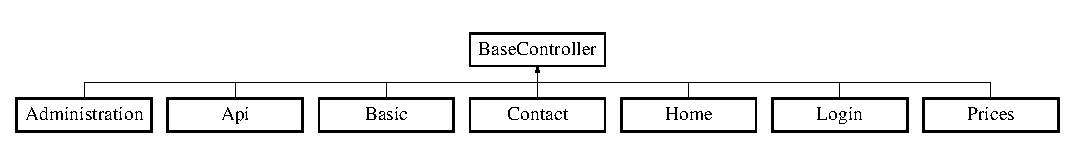
\includegraphics[height=2.000000cm]{class_base_controller}
\end{center}
\end{figure}
\subsection*{Public Member Functions}
\begin{DoxyCompactItemize}
\item 
\hyperlink{class_base_controller_a095c5d389db211932136b53f25f39685}{\+\_\+\+\_\+construct} ()
\end{DoxyCompactItemize}
\subsection*{Protected Member Functions}
\begin{DoxyCompactItemize}
\item 
\hyperlink{class_base_controller_a5fa8890bd3a9d20f5c0cc2377dc49eb1}{load\+Model} (\$model, \$constructor=\mbox{[}$\,$\mbox{]})
\item 
\hyperlink{class_base_controller_a170629218b28c1759a89c4978b9323b3}{post\+Input} (\$input=null)
\item 
\hyperlink{class_base_controller_aa0c49b95cd8e5ff8ff61b4a2c35bf1eb}{render\+View} (\$view, \$data=\mbox{[}$\,$\mbox{]})
\item 
\hyperlink{class_base_controller_abd4f25604b09a96c254491df97612cc3}{scrape} (\$action, \$url, \$curl=null)
\item 
\hyperlink{class_base_controller_a259a554926fc05640c8c711c340cdeac}{session} (\$url, \$post\+Data)
\end{DoxyCompactItemize}


\subsection{Detailed Description}


Definition at line 3 of file Base\+Controller.\+php.



\subsection{Constructor \& Destructor Documentation}
\hypertarget{class_base_controller_a095c5d389db211932136b53f25f39685}{}\label{class_base_controller_a095c5d389db211932136b53f25f39685} 
\index{Base\+Controller@{Base\+Controller}!\+\_\+\+\_\+construct@{\+\_\+\+\_\+construct}}
\index{\+\_\+\+\_\+construct@{\+\_\+\+\_\+construct}!Base\+Controller@{Base\+Controller}}
\subsubsection{\texorpdfstring{\+\_\+\+\_\+construct()}{\_\_construct()}}
{\footnotesize\ttfamily \+\_\+\+\_\+construct (\begin{DoxyParamCaption}{ }\end{DoxyParamCaption})}



Definition at line 4 of file Base\+Controller.\+php.



References E\+R\+R\+O\+R\+\_\+\+R\+E\+P\+O\+R\+T\+I\+NG.


\begin{DoxyCode}
4                                   \{
5         error\_reporting(\hyperlink{config_8php_a80c2f40a4ce1ad3cbfb1978239f63c31}{ERROR\_REPORTING});
6     \}
\end{DoxyCode}


\subsection{Member Function Documentation}
\hypertarget{class_base_controller_a5fa8890bd3a9d20f5c0cc2377dc49eb1}{}\label{class_base_controller_a5fa8890bd3a9d20f5c0cc2377dc49eb1} 
\index{Base\+Controller@{Base\+Controller}!load\+Model@{load\+Model}}
\index{load\+Model@{load\+Model}!Base\+Controller@{Base\+Controller}}
\subsubsection{\texorpdfstring{load\+Model()}{loadModel()}}
{\footnotesize\ttfamily load\+Model (\begin{DoxyParamCaption}\item[{}]{\$model,  }\item[{}]{\$constructor = {\ttfamily \mbox{[}\mbox{]}} }\end{DoxyParamCaption})\hspace{0.3cm}{\ttfamily [protected]}}

Loads a given model into the controller


\begin{DoxyParams}[1]{Parameters}
string & {\em \$model} & \\
\hline
array & {\em \$constructor} & \\
\hline
\end{DoxyParams}
\begin{DoxyReturn}{Returns}
object \$model 
\end{DoxyReturn}


Definition at line 15 of file Base\+Controller.\+php.



Referenced by Basic\textbackslash{}create\+User(), Basic\textbackslash{}delete\+User(), Basic\textbackslash{}edit\+User(), Basic\textbackslash{}edit\+User\+Post(), Basic\textbackslash{}index(), Basic\textbackslash{}return\+Model(), and Basic\textbackslash{}user().


\begin{DoxyCode}
15                                                             \{
16         \textcolor{keywordflow}{if} (file\_exists(realpath(\_\_DIR\_\_ . \textcolor{stringliteral}{'/..'}) . \textcolor{stringliteral}{'/models/'} . $model . \textcolor{stringliteral}{'.php'})) \{
17             require\_once realpath(\_\_DIR\_\_ . \textcolor{stringliteral}{'/..'}) . \textcolor{stringliteral}{'/models/'} . $model . \textcolor{stringliteral}{'.php'};
18         \}
19         \textcolor{keywordflow}{else} \{
20             \textcolor{keywordflow}{throw} \textcolor{keyword}{new} \hyperlink{class_model_not_found}{ModelNotFound}(\textcolor{stringliteral}{'ModelNotFound'}, \textcolor{stringliteral}{'Model "'} . $model . \textcolor{stringliteral}{'" not found.'});
21             exit();
22         \}
23 
24         \textcolor{keywordflow}{return} \textcolor{keyword}{new} $model($constructor);
25     \}
\end{DoxyCode}
\hypertarget{class_base_controller_a170629218b28c1759a89c4978b9323b3}{}\label{class_base_controller_a170629218b28c1759a89c4978b9323b3} 
\index{Base\+Controller@{Base\+Controller}!post\+Input@{post\+Input}}
\index{post\+Input@{post\+Input}!Base\+Controller@{Base\+Controller}}
\subsubsection{\texorpdfstring{post\+Input()}{postInput()}}
{\footnotesize\ttfamily post\+Input (\begin{DoxyParamCaption}\item[{}]{\$input = {\ttfamily null} }\end{DoxyParamCaption})\hspace{0.3cm}{\ttfamily [protected]}}

Sanitizes and returns P\+O\+ST data


\begin{DoxyParams}[1]{Parameters}
string & {\em \$input} & \\
\hline
\end{DoxyParams}
\begin{DoxyReturn}{Returns}
string/array 
\end{DoxyReturn}


Definition at line 33 of file Base\+Controller.\+php.



Referenced by Basic\textbackslash{}create\+User(), and Basic\textbackslash{}edit\+User\+Post().


\begin{DoxyCode}
33                                                 \{
34         $post = filter\_input\_array(INPUT\_POST, FILTER\_SANITIZE\_STRING);
35 
36         \textcolor{keywordflow}{if} ($input) \{
37             \textcolor{keywordflow}{return} $post[$input];
38         \}
39         \textcolor{keywordflow}{else} \{
40             \textcolor{keywordflow}{return} $post;
41         \}
42     \}
\end{DoxyCode}
\hypertarget{class_base_controller_aa0c49b95cd8e5ff8ff61b4a2c35bf1eb}{}\label{class_base_controller_aa0c49b95cd8e5ff8ff61b4a2c35bf1eb} 
\index{Base\+Controller@{Base\+Controller}!render\+View@{render\+View}}
\index{render\+View@{render\+View}!Base\+Controller@{Base\+Controller}}
\subsubsection{\texorpdfstring{render\+View()}{renderView()}}
{\footnotesize\ttfamily render\+View (\begin{DoxyParamCaption}\item[{}]{\$view,  }\item[{}]{\$data = {\ttfamily \mbox{[}\mbox{]}} }\end{DoxyParamCaption})\hspace{0.3cm}{\ttfamily [protected]}}

Loads a given view into the controller


\begin{DoxyParams}[1]{Parameters}
string & {\em \$view} & \\
\hline
array & {\em \$data} & \\
\hline
\end{DoxyParams}


Definition at line 50 of file Base\+Controller.\+php.



Referenced by Basic\textbackslash{}edit\+User(), Basic\textbackslash{}index(), and Basic\textbackslash{}user().


\begin{DoxyCode}
50                                                      \{
51         $loader = \textcolor{keyword}{new} Twig\_Loader\_Filesystem(realpath(\_\_DIR\_\_ . \textcolor{stringliteral}{'/..'}) . \textcolor{stringliteral}{'/views'});
52         $twig = \textcolor{keyword}{new} Twig\_Environment($loader, [
53             \textcolor{stringliteral}{'debug'} => \textcolor{keyword}{true},
54             ]);
55         $twig->addExtension(\textcolor{keyword}{new} Twig\_Extension\_Debug());
56 
57         \textcolor{keywordflow}{return} $twig->render($view . \textcolor{stringliteral}{'.php'}, [
58             \textcolor{stringliteral}{'data'} => $data
59             ]);
60     \}
\end{DoxyCode}
\hypertarget{class_base_controller_abd4f25604b09a96c254491df97612cc3}{}\label{class_base_controller_abd4f25604b09a96c254491df97612cc3} 
\index{Base\+Controller@{Base\+Controller}!scrape@{scrape}}
\index{scrape@{scrape}!Base\+Controller@{Base\+Controller}}
\subsubsection{\texorpdfstring{scrape()}{scrape()}}
{\footnotesize\ttfamily scrape (\begin{DoxyParamCaption}\item[{}]{\$action,  }\item[{}]{\$url,  }\item[{}]{\$curl = {\ttfamily null} }\end{DoxyParamCaption})\hspace{0.3cm}{\ttfamily [protected]}}

Scrapes H\+T\+ML source code from the given U\+RL


\begin{DoxyParams}[1]{Parameters}
string & {\em \$url} & \\
\hline
string & {\em \$action} & \\
\hline
curl & {\em \$curl} & \\
\hline
\end{DoxyParams}
\begin{DoxyReturn}{Returns}
string \$html 
\end{DoxyReturn}


Definition at line 70 of file Base\+Controller.\+php.



References str\+\_\+get\+\_\+html().



Referenced by Basic\textbackslash{}scrape\+Pdf(), and Basic\textbackslash{}scrape\+Website().


\begin{DoxyCode}
70                                                            \{
71         \textcolor{keywordflow}{switch} (strtoupper($action)) \{
72             \textcolor{keywordflow}{case} \textcolor{stringliteral}{'GET'}:
73             $html = \textcolor{keyword}{new} \hyperlink{classsimple__html__dom}{simple\_html\_dom}();
74             \textcolor{keywordflow}{if} ($curl) \{
75                 curl\_setopt($curl, CURLOPT\_RETURNTRANSFER, 1); 
76                 curl\_setopt($curl, CURLOPT\_POST, 0);
77                 curl\_setopt($curl, CURLOPT\_URL, $url);
78                 $html = \hyperlink{simple__html__dom_8php_a2a9c7626f0cb0a56eb81709124a08922}{str\_get\_html}(curl\_exec($curl));
79                 curl\_close($curl);
80             \}
81             \textcolor{keywordflow}{else} \{
82                 $html->load\_file($url);
83             \}
84             \textcolor{keywordflow}{return} $html;
85             \textcolor{keywordflow}{break};
86             
87             \textcolor{keywordflow}{case} \textcolor{stringliteral}{'PDF'}:
88             $parser = \textcolor{keyword}{new} Parser();
89             $pdf = $parser->parseFile($url);
90 
91             \textcolor{keywordflow}{return} $pdf;
92             \textcolor{keywordflow}{break};
93         \}
94     \}
\end{DoxyCode}
\hypertarget{class_base_controller_a259a554926fc05640c8c711c340cdeac}{}\label{class_base_controller_a259a554926fc05640c8c711c340cdeac} 
\index{Base\+Controller@{Base\+Controller}!session@{session}}
\index{session@{session}!Base\+Controller@{Base\+Controller}}
\subsubsection{\texorpdfstring{session()}{session()}}
{\footnotesize\ttfamily session (\begin{DoxyParamCaption}\item[{}]{\$url,  }\item[{}]{\$post\+Data }\end{DoxyParamCaption})\hspace{0.3cm}{\ttfamily [protected]}}

Initializes session with c\+U\+RL and saves session cookies in file for later retrieval


\begin{DoxyParams}[1]{Parameters}
string & {\em \$url} & \\
\hline
array & {\em \$post\+Data} & \\
\hline
\end{DoxyParams}
\begin{DoxyReturn}{Returns}
\$curl 
\end{DoxyReturn}


Definition at line 103 of file Base\+Controller.\+php.


\begin{DoxyCode}
103                                                 \{
104         $curl = curl\_init();
105 
106         curl\_setopt($curl, CURLOPT\_RETURNTRANSFER, 1); 
107 
108         curl\_setopt($curl, CURLOPT\_URL, $url);
109         $cookie = dirname(\_\_FILE\_\_) . \textcolor{stringliteral}{'/cookies.txt'};
110         $timeout = 30;
111 
112         curl\_setopt($curl, CURLOPT\_USERAGENT, \textcolor{stringliteral}{'Mozilla/5.0 (Windows NT 6.1; WOW64) AppleWebKit/537.36
       (KHTML, like Gecko) Chrome/54.0.2840.71 Safari/537.36'});
113         curl\_setopt($curl, CURLOPT\_FOLLOWLOCATION, 1);
114         curl\_setopt($curl, CURLOPT\_TIMEOUT, 10); 
115         curl\_setopt($curl, CURLOPT\_CONNECTTIMEOUT, $timeout);
116         curl\_setopt($curl, CURLOPT\_COOKIEJAR, $cookie);
117         curl\_setopt($curl, CURLOPT\_COOKIEFILE, $cookie);
118 
119         curl\_setopt($curl, CURLOPT\_POST, 1); 
120         curl\_setopt($curl, CURLOPT\_POSTFIELDS, http\_build\_query($postData));     
121         curl\_setopt($curl, CURLOPT\_SSL\_VERIFYPEER, 0);
122         unlink($cookie);
123         curl\_exec($curl);
124 
125         \textcolor{keywordflow}{return} $curl;
126     \}
\end{DoxyCode}


The documentation for this class was generated from the following file\+:\begin{DoxyCompactItemize}
\item 
C\+:/xampp/htdocs/mvc-\/framework/application/kernel/\hyperlink{_base_controller_8php}{Base\+Controller.\+php}\end{DoxyCompactItemize}

\hypertarget{class_basic}{}\section{Basic Class Reference}
\label{class_basic}\index{Basic@{Basic}}
Inheritance diagram for Basic\+:\begin{figure}[H]
\begin{center}
\leavevmode
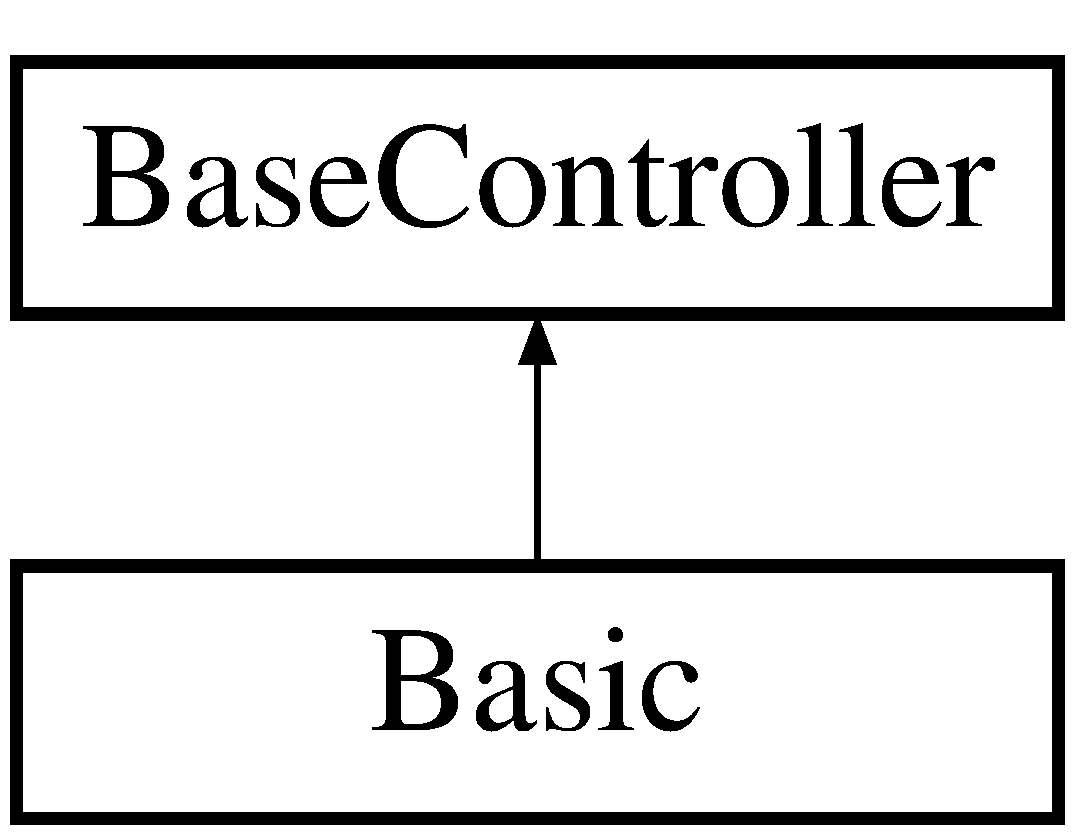
\includegraphics[height=2.000000cm]{class_basic}
\end{center}
\end{figure}
\subsection*{Public Member Functions}
\begin{DoxyCompactItemize}
\item 
\hyperlink{class_basic_a149eb92716c1084a935e04a8d95f7347}{index} ()
\item 
\hyperlink{class_basic_a6603546e99f9519b86989be128736ad6}{user} (\$id=\textquotesingle{}\textquotesingle{})
\item 
\hyperlink{class_basic_a48ffe9a27b91ce968b2bcf5e0a9d4069}{scrape\+Website} ()
\item 
\hyperlink{class_basic_a7cb6a02987f0faaef2ee4aff9198907e}{return\+Model} ()
\item 
\hyperlink{class_basic_a16df2136bd66a75022f350d583e6c060}{return\+Hash} ()
\item 
\hyperlink{class_basic_a967982ee98f05287bbdba812f6016947}{create\+User} ()
\item 
\hyperlink{class_basic_acd3b430aeceba0ebbda62330838d0c0b}{edit\+User} (\$id=\textquotesingle{}\textquotesingle{})
\item 
\hyperlink{class_basic_a445a1f2f42c756bf451de087e36b7193}{edit\+User\+Post} ()
\item 
\hyperlink{class_basic_a934aeeec370d904f3a58bde4d514259d}{delete\+User} (\$id=\textquotesingle{}\textquotesingle{})
\item 
\hyperlink{class_basic_a1f753d67be418d065282360fc5231d05}{send\+Mail} ()
\item 
\hyperlink{class_basic_a624b6482127c1e3ea78392e7e93db949}{send\+S\+MS} ()
\item 
\hyperlink{class_basic_a5bb666dcea19a9561c2047cfa25936bd}{return\+String} ()
\item 
\hyperlink{class_basic_a8d2918087022004ef5ad62d8f76a73d7}{return\+Int} ()
\item 
\hyperlink{class_basic_abf786273f796a96f5532dc60f9cec813}{redirect\+To\+Url} ()
\item 
\hyperlink{class_basic_a53f01fc4c43d1cecc497d9645f920407}{redirect\+To\+Controller} ()
\item 
\hyperlink{class_basic_ac380e8a432563c6affcfddd43384c1d2}{return\+Parameter} (\$parameter=\textquotesingle{}\textquotesingle{})
\item 
\hyperlink{class_basic_a2ef87b96abcca966a41e34d077fcc38e}{return\+Two\+Parameters} (\$parameter1=\textquotesingle{}\textquotesingle{}, \$parameter2=\textquotesingle{}\textquotesingle{})
\end{DoxyCompactItemize}
\subsection*{Additional Inherited Members}


\subsection{Detailed Description}


Definition at line 5 of file Basic.\+php.



\subsection{Member Function Documentation}
\hypertarget{class_basic_a967982ee98f05287bbdba812f6016947}{}\label{class_basic_a967982ee98f05287bbdba812f6016947} 
\index{Basic@{Basic}!create\+User@{create\+User}}
\index{create\+User@{create\+User}!Basic@{Basic}}
\subsubsection{\texorpdfstring{create\+User()}{createUser()}}
{\footnotesize\ttfamily create\+User (\begin{DoxyParamCaption}{ }\end{DoxyParamCaption})}



Definition at line 35 of file Basic.\+php.



References Base\+Controller\textbackslash{}load\+Model(), Base\+Controller\textbackslash{}post\+Input(), and Base\+Controller\textbackslash{}redirect\+Controller().


\begin{DoxyCode}
35                                  \{
36         $postInput = $this->\hyperlink{class_base_controller_a170629218b28c1759a89c4978b9323b3}{postInput}();
37 
38         $user = $this->\hyperlink{class_base_controller_a5fa8890bd3a9d20f5c0cc2377dc49eb1}{loadModel}(\textcolor{stringliteral}{'Users'});
39         Users::create($postInput);
40 
41         $this->\hyperlink{class_base_controller_a85ddb683efc64655be063b697f631beb}{redirectController}(\textcolor{stringliteral}{'Basic'});
42     \}
\end{DoxyCode}
\hypertarget{class_basic_a934aeeec370d904f3a58bde4d514259d}{}\label{class_basic_a934aeeec370d904f3a58bde4d514259d} 
\index{Basic@{Basic}!delete\+User@{delete\+User}}
\index{delete\+User@{delete\+User}!Basic@{Basic}}
\subsubsection{\texorpdfstring{delete\+User()}{deleteUser()}}
{\footnotesize\ttfamily delete\+User (\begin{DoxyParamCaption}\item[{}]{\$id = {\ttfamily \textquotesingle{}\textquotesingle{}} }\end{DoxyParamCaption})}



Definition at line 63 of file Basic.\+php.



References Base\+Controller\textbackslash{}load\+Model(), and Base\+Controller\textbackslash{}redirect\+Controller().


\begin{DoxyCode}
63                                          \{
64         $user = $this->\hyperlink{class_base_controller_a5fa8890bd3a9d20f5c0cc2377dc49eb1}{loadModel}(\textcolor{stringliteral}{'Users'});
65         $user = Users::find($id);
66         $user->delete();
67 
68         $this->\hyperlink{class_base_controller_a85ddb683efc64655be063b697f631beb}{redirectController}(\textcolor{stringliteral}{'Basic'});
69     \}
\end{DoxyCode}
\hypertarget{class_basic_acd3b430aeceba0ebbda62330838d0c0b}{}\label{class_basic_acd3b430aeceba0ebbda62330838d0c0b} 
\index{Basic@{Basic}!edit\+User@{edit\+User}}
\index{edit\+User@{edit\+User}!Basic@{Basic}}
\subsubsection{\texorpdfstring{edit\+User()}{editUser()}}
{\footnotesize\ttfamily edit\+User (\begin{DoxyParamCaption}\item[{}]{\$id = {\ttfamily \textquotesingle{}\textquotesingle{}} }\end{DoxyParamCaption})}



Definition at line 43 of file Basic.\+php.



References Base\+Controller\textbackslash{}load\+Model(), and Base\+Controller\textbackslash{}render\+View().


\begin{DoxyCode}
43                                        \{
44         $user = $this->\hyperlink{class_base_controller_a5fa8890bd3a9d20f5c0cc2377dc49eb1}{loadModel}(\textcolor{stringliteral}{'Users'});
45         $user = Users::find($id);
46 
47         echo $this->\hyperlink{class_base_controller_aa0c49b95cd8e5ff8ff61b4a2c35bf1eb}{renderView}(\textcolor{stringliteral}{'layout/basic\_edit'}, [\textcolor{stringliteral}{'user'} => $user]);
48     \}
\end{DoxyCode}
\hypertarget{class_basic_a445a1f2f42c756bf451de087e36b7193}{}\label{class_basic_a445a1f2f42c756bf451de087e36b7193} 
\index{Basic@{Basic}!edit\+User\+Post@{edit\+User\+Post}}
\index{edit\+User\+Post@{edit\+User\+Post}!Basic@{Basic}}
\subsubsection{\texorpdfstring{edit\+User\+Post()}{editUserPost()}}
{\footnotesize\ttfamily edit\+User\+Post (\begin{DoxyParamCaption}{ }\end{DoxyParamCaption})}



Definition at line 49 of file Basic.\+php.



References Base\+Controller\textbackslash{}load\+Model(), Base\+Controller\textbackslash{}post\+Input(), and Base\+Controller\textbackslash{}redirect\+Controller().


\begin{DoxyCode}
49                                    \{
50         $user = $this->\hyperlink{class_base_controller_a5fa8890bd3a9d20f5c0cc2377dc49eb1}{loadModel}(\textcolor{stringliteral}{'Users'});
51         $user = Users::find($this->\hyperlink{class_base_controller_a170629218b28c1759a89c4978b9323b3}{postInput}(\textcolor{stringliteral}{'id'}));
52 
53         $user->firstName = $this->\hyperlink{class_base_controller_a170629218b28c1759a89c4978b9323b3}{postInput}(\textcolor{stringliteral}{'firstName'});
54         $user->lastName = $this->\hyperlink{class_base_controller_a170629218b28c1759a89c4978b9323b3}{postInput}(\textcolor{stringliteral}{'lastName'});
55         $user->age = $this->\hyperlink{class_base_controller_a170629218b28c1759a89c4978b9323b3}{postInput}(\textcolor{stringliteral}{'age'});
56         $user->avatar = $this->\hyperlink{class_base_controller_a170629218b28c1759a89c4978b9323b3}{postInput}(\textcolor{stringliteral}{'avatar'});
57         $user->email = $this->\hyperlink{class_base_controller_a170629218b28c1759a89c4978b9323b3}{postInput}(\textcolor{stringliteral}{'email'});
58         $user->phone = $this->\hyperlink{class_base_controller_a170629218b28c1759a89c4978b9323b3}{postInput}(\textcolor{stringliteral}{'phone'});
59         $user->save();
60 
61         $this->\hyperlink{class_base_controller_a85ddb683efc64655be063b697f631beb}{redirectController}(\textcolor{stringliteral}{'Basic'});
62     \}
\end{DoxyCode}
\hypertarget{class_basic_a149eb92716c1084a935e04a8d95f7347}{}\label{class_basic_a149eb92716c1084a935e04a8d95f7347} 
\index{Basic@{Basic}!index@{index}}
\index{index@{index}!Basic@{Basic}}
\subsubsection{\texorpdfstring{index()}{index()}}
{\footnotesize\ttfamily index (\begin{DoxyParamCaption}{ }\end{DoxyParamCaption})}



Definition at line 6 of file Basic.\+php.



References Base\+Controller\textbackslash{}load\+Model(), and Base\+Controller\textbackslash{}render\+View().


\begin{DoxyCode}
6                             \{
7         $users = $this->\hyperlink{class_base_controller_a5fa8890bd3a9d20f5c0cc2377dc49eb1}{loadModel}(\textcolor{stringliteral}{'Users'});
8         $users = Users::all()->sortBy(\textcolor{stringliteral}{'firstName'});
9 
10         echo $this->\hyperlink{class_base_controller_aa0c49b95cd8e5ff8ff61b4a2c35bf1eb}{renderView}(\textcolor{stringliteral}{'layout/basic'}, [\textcolor{stringliteral}{'userArray'} => $users]);
11     \}
\end{DoxyCode}
\hypertarget{class_basic_a53f01fc4c43d1cecc497d9645f920407}{}\label{class_basic_a53f01fc4c43d1cecc497d9645f920407} 
\index{Basic@{Basic}!redirect\+To\+Controller@{redirect\+To\+Controller}}
\index{redirect\+To\+Controller@{redirect\+To\+Controller}!Basic@{Basic}}
\subsubsection{\texorpdfstring{redirect\+To\+Controller()}{redirectToController()}}
{\footnotesize\ttfamily redirect\+To\+Controller (\begin{DoxyParamCaption}{ }\end{DoxyParamCaption})}



Definition at line 105 of file Basic.\+php.



References Base\+Controller\textbackslash{}redirect\+Controller().


\begin{DoxyCode}
105                                            \{
106         $this->\hyperlink{class_base_controller_a85ddb683efc64655be063b697f631beb}{redirectController}(\textcolor{stringliteral}{'Basic'});
107     \}
\end{DoxyCode}
\hypertarget{class_basic_abf786273f796a96f5532dc60f9cec813}{}\label{class_basic_abf786273f796a96f5532dc60f9cec813} 
\index{Basic@{Basic}!redirect\+To\+Url@{redirect\+To\+Url}}
\index{redirect\+To\+Url@{redirect\+To\+Url}!Basic@{Basic}}
\subsubsection{\texorpdfstring{redirect\+To\+Url()}{redirectToUrl()}}
{\footnotesize\ttfamily redirect\+To\+Url (\begin{DoxyParamCaption}{ }\end{DoxyParamCaption})}



Definition at line 102 of file Basic.\+php.



References Base\+Controller\textbackslash{}redirect\+Url().


\begin{DoxyCode}
102                                     \{
103         $this->\hyperlink{class_base_controller_a9f95c7503770ed9c974005b363ec3d00}{redirectUrl}(\_\_DIR\_\_ . \textcolor{stringliteral}{'/returnString'});
104     \}
\end{DoxyCode}
\hypertarget{class_basic_a16df2136bd66a75022f350d583e6c060}{}\label{class_basic_a16df2136bd66a75022f350d583e6c060} 
\index{Basic@{Basic}!return\+Hash@{return\+Hash}}
\index{return\+Hash@{return\+Hash}!Basic@{Basic}}
\subsubsection{\texorpdfstring{return\+Hash()}{returnHash()}}
{\footnotesize\ttfamily return\+Hash (\begin{DoxyParamCaption}{ }\end{DoxyParamCaption})}



Definition at line 32 of file Basic.\+php.



References Base\+Controller\textbackslash{}hash\+String().


\begin{DoxyCode}
32                                  \{
33         \textcolor{keywordflow}{return} $this->\hyperlink{class_base_controller_ac7f37d2e13bade1709f5c88b02f0e9d1}{hashString}(\textcolor{stringliteral}{'daniel'});
34     \}
\end{DoxyCode}
\hypertarget{class_basic_a8d2918087022004ef5ad62d8f76a73d7}{}\label{class_basic_a8d2918087022004ef5ad62d8f76a73d7} 
\index{Basic@{Basic}!return\+Int@{return\+Int}}
\index{return\+Int@{return\+Int}!Basic@{Basic}}
\subsubsection{\texorpdfstring{return\+Int()}{returnInt()}}
{\footnotesize\ttfamily return\+Int (\begin{DoxyParamCaption}{ }\end{DoxyParamCaption})}



Definition at line 99 of file Basic.\+php.


\begin{DoxyCode}
99                                 \{
100         \textcolor{keywordflow}{return} 24;
101     \}
\end{DoxyCode}
\hypertarget{class_basic_a7cb6a02987f0faaef2ee4aff9198907e}{}\label{class_basic_a7cb6a02987f0faaef2ee4aff9198907e} 
\index{Basic@{Basic}!return\+Model@{return\+Model}}
\index{return\+Model@{return\+Model}!Basic@{Basic}}
\subsubsection{\texorpdfstring{return\+Model()}{returnModel()}}
{\footnotesize\ttfamily return\+Model (\begin{DoxyParamCaption}{ }\end{DoxyParamCaption})}



Definition at line 26 of file Basic.\+php.



References Base\+Controller\textbackslash{}load\+Model().


\begin{DoxyCode}
26                                   \{
27         $user = $this->\hyperlink{class_base_controller_a5fa8890bd3a9d20f5c0cc2377dc49eb1}{loadModel}(\textcolor{stringliteral}{'User'});
28         $user->setFirstName(\textcolor{stringliteral}{'daniel'});
29 
30         \textcolor{keywordflow}{return} $user;
31     \}
\end{DoxyCode}
\hypertarget{class_basic_ac380e8a432563c6affcfddd43384c1d2}{}\label{class_basic_ac380e8a432563c6affcfddd43384c1d2} 
\index{Basic@{Basic}!return\+Parameter@{return\+Parameter}}
\index{return\+Parameter@{return\+Parameter}!Basic@{Basic}}
\subsubsection{\texorpdfstring{return\+Parameter()}{returnParameter()}}
{\footnotesize\ttfamily return\+Parameter (\begin{DoxyParamCaption}\item[{}]{\$parameter = {\ttfamily \textquotesingle{}\textquotesingle{}} }\end{DoxyParamCaption})}



Definition at line 108 of file Basic.\+php.


\begin{DoxyCode}
108                                                      \{
109         \textcolor{keywordflow}{return} $parameter;
110     \}
\end{DoxyCode}
\hypertarget{class_basic_a5bb666dcea19a9561c2047cfa25936bd}{}\label{class_basic_a5bb666dcea19a9561c2047cfa25936bd} 
\index{Basic@{Basic}!return\+String@{return\+String}}
\index{return\+String@{return\+String}!Basic@{Basic}}
\subsubsection{\texorpdfstring{return\+String()}{returnString()}}
{\footnotesize\ttfamily return\+String (\begin{DoxyParamCaption}{ }\end{DoxyParamCaption})}



Definition at line 96 of file Basic.\+php.


\begin{DoxyCode}
96                                    \{
97         \textcolor{keywordflow}{return} \textcolor{stringliteral}{'daniel'};
98     \}
\end{DoxyCode}
\hypertarget{class_basic_a2ef87b96abcca966a41e34d077fcc38e}{}\label{class_basic_a2ef87b96abcca966a41e34d077fcc38e} 
\index{Basic@{Basic}!return\+Two\+Parameters@{return\+Two\+Parameters}}
\index{return\+Two\+Parameters@{return\+Two\+Parameters}!Basic@{Basic}}
\subsubsection{\texorpdfstring{return\+Two\+Parameters()}{returnTwoParameters()}}
{\footnotesize\ttfamily return\+Two\+Parameters (\begin{DoxyParamCaption}\item[{}]{\$parameter1 = {\ttfamily \textquotesingle{}\textquotesingle{}},  }\item[{}]{\$parameter2 = {\ttfamily \textquotesingle{}\textquotesingle{}} }\end{DoxyParamCaption})}



Definition at line 111 of file Basic.\+php.


\begin{DoxyCode}
111                                                                             \{
112         \textcolor{keywordflow}{return} $parameter1 . $parameter2;
113     \}
\end{DoxyCode}
\hypertarget{class_basic_a48ffe9a27b91ce968b2bcf5e0a9d4069}{}\label{class_basic_a48ffe9a27b91ce968b2bcf5e0a9d4069} 
\index{Basic@{Basic}!scrape\+Website@{scrape\+Website}}
\index{scrape\+Website@{scrape\+Website}!Basic@{Basic}}
\subsubsection{\texorpdfstring{scrape\+Website()}{scrapeWebsite()}}
{\footnotesize\ttfamily scrape\+Website (\begin{DoxyParamCaption}{ }\end{DoxyParamCaption})}



Definition at line 18 of file Basic.\+php.



References Base\+Controller\textbackslash{}scrape().


\begin{DoxyCode}
18                                     \{
19         \textcolor{comment}{/*$curl = $this->session('https://m.facebook.com/login.php', ['email' => '', 'pass' => '',
       '\_fb\_noscript' => 'true']);}
20 \textcolor{comment}{        $html = $this->scrape('GET', 'https://m.facebook.com/danieldk1992/friends/', $curl);*/}
21 
22         $html = $this->\hyperlink{class_base_controller_abd4f25604b09a96c254491df97612cc3}{scrape}(\textcolor{stringliteral}{'GET'}, \textcolor{stringliteral}{'http://ekstrabladet.dk/'});
23 
24         \textcolor{keywordflow}{return} $html->getElementByTagName(\textcolor{stringliteral}{'title'})->plaintext;
25     \}
\end{DoxyCode}
\hypertarget{class_basic_a1f753d67be418d065282360fc5231d05}{}\label{class_basic_a1f753d67be418d065282360fc5231d05} 
\index{Basic@{Basic}!send\+Mail@{send\+Mail}}
\index{send\+Mail@{send\+Mail}!Basic@{Basic}}
\subsubsection{\texorpdfstring{send\+Mail()}{sendMail()}}
{\footnotesize\ttfamily send\+Mail (\begin{DoxyParamCaption}{ }\end{DoxyParamCaption})}



Definition at line 70 of file Basic.\+php.



References initialize\+Config().


\begin{DoxyCode}
70                                \{
71         $config = \hyperlink{config_8php_afeb1d281d402615776fdb0320a5b8d05}{initializeConfig}();
72         $mgClient = \textcolor{keyword}{new} Mailgun($config[\textcolor{stringliteral}{'mailgunKey'}]);
73         $domain = $config[\textcolor{stringliteral}{'mailgunDomain'}];
74 
75         $result = $mgClient->sendMessage($domain,
76             array(\textcolor{stringliteral}{'from'}    => \textcolor{stringliteral}{'Mailgun Sandbox
       <postmaster@sandbox5c2500d99acf4cbfa26fa88a596a49bd.mailgun.org>'},
77                 \textcolor{stringliteral}{'to'}      => \textcolor{stringliteral}{'Daniel Winther Jensen <danielwinther@hotmail.dk>'},
78                 \textcolor{stringliteral}{'subject'} => \textcolor{stringliteral}{'Hello Daniel Winther Jensen'},
79                 \textcolor{stringliteral}{'text'}    => \textcolor{stringliteral}{'Congratulations Daniel Winther Jensen, you just sent an email with Mailgun! 
       You are truly awesome!  You can see a record of this email in your logs: https://mailgun.com/cp/log .  You
       can send up to 300 emails/day from this sandbox server.  Next, you should add your own domain so you can send
       10,000 emails/month for free.'}));
80     \}
\end{DoxyCode}
\hypertarget{class_basic_a624b6482127c1e3ea78392e7e93db949}{}\label{class_basic_a624b6482127c1e3ea78392e7e93db949} 
\index{Basic@{Basic}!send\+S\+MS@{send\+S\+MS}}
\index{send\+S\+MS@{send\+S\+MS}!Basic@{Basic}}
\subsubsection{\texorpdfstring{send\+S\+M\+S()}{sendSMS()}}
{\footnotesize\ttfamily send\+S\+MS (\begin{DoxyParamCaption}{ }\end{DoxyParamCaption})}



Definition at line 81 of file Basic.\+php.



References initialize\+Config().


\begin{DoxyCode}
81                               \{
82         $config = \hyperlink{config_8php_afeb1d281d402615776fdb0320a5b8d05}{initializeConfig}();
83         $sid = $config[\textcolor{stringliteral}{'twilioSid'}];
84         $token = $config[\textcolor{stringliteral}{'twilioToken'}];
85         $client = \textcolor{keyword}{new} Client($sid, $token);
86 
87         $client->messages->create(
88             \textcolor{stringliteral}{'+4542341338'},
89             array(
90                 \textcolor{stringliteral}{'from'} => \textcolor{stringliteral}{'+46769447755'},
91                 \textcolor{stringliteral}{'body'} => \textcolor{stringliteral}{'This is a test'}
92                 )
93             );
94     \}
\end{DoxyCode}
\hypertarget{class_basic_a6603546e99f9519b86989be128736ad6}{}\label{class_basic_a6603546e99f9519b86989be128736ad6} 
\index{Basic@{Basic}!user@{user}}
\index{user@{user}!Basic@{Basic}}
\subsubsection{\texorpdfstring{user()}{user()}}
{\footnotesize\ttfamily user (\begin{DoxyParamCaption}\item[{}]{\$id = {\ttfamily \textquotesingle{}\textquotesingle{}} }\end{DoxyParamCaption})}



Definition at line 12 of file Basic.\+php.



References Base\+Controller\textbackslash{}load\+Model(), and Base\+Controller\textbackslash{}render\+View().


\begin{DoxyCode}
12                                    \{
13         $user = $this->\hyperlink{class_base_controller_a5fa8890bd3a9d20f5c0cc2377dc49eb1}{loadModel}(\textcolor{stringliteral}{'Users'});
14         $user = Users::find($id);
15 
16         echo $this->\hyperlink{class_base_controller_aa0c49b95cd8e5ff8ff61b4a2c35bf1eb}{renderView}(\textcolor{stringliteral}{'layout/basic\_detail'}, [\textcolor{stringliteral}{'user'} => $user]);
17     \}
\end{DoxyCode}


The documentation for this class was generated from the following file\+:\begin{DoxyCompactItemize}
\item 
C\+:/xampp/htdocs/mvc-\/framework/application/controllers/\hyperlink{controllers_2_basic_8php}{Basic.\+php}\end{DoxyCompactItemize}

\hypertarget{class_controller_not_found}{}\section{Controller\+Not\+Found Class Reference}
\label{class_controller_not_found}\index{Controller\+Not\+Found@{Controller\+Not\+Found}}
Inheritance diagram for Controller\+Not\+Found\+:\begin{figure}[H]
\begin{center}
\leavevmode
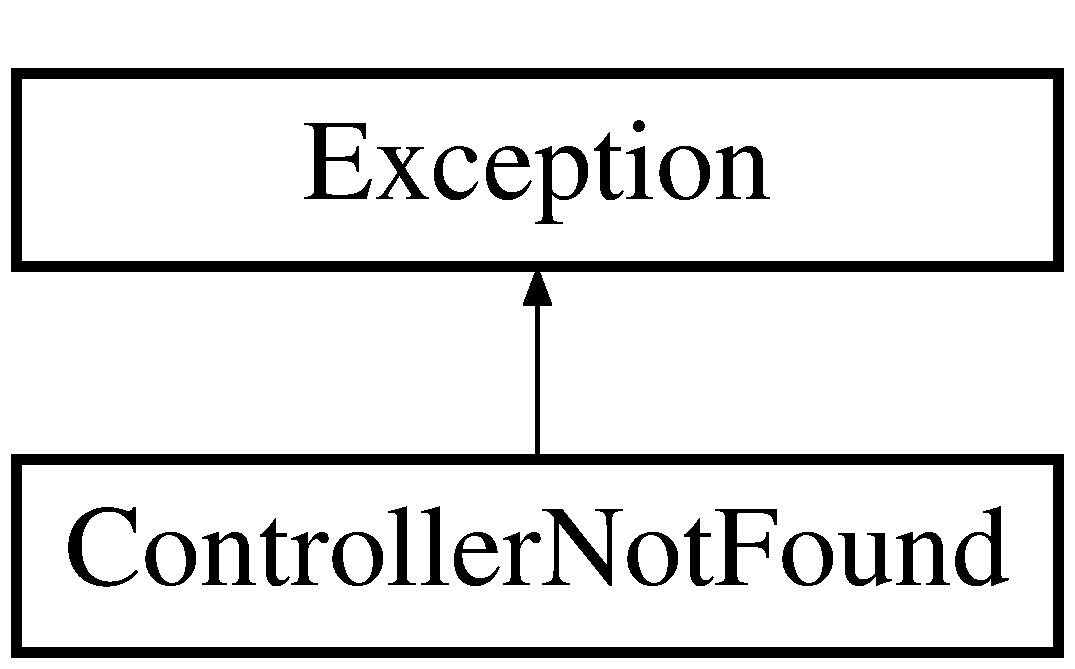
\includegraphics[height=2.000000cm]{class_controller_not_found}
\end{center}
\end{figure}
\subsection*{Public Member Functions}
\begin{DoxyCompactItemize}
\item 
\hyperlink{class_controller_not_found_a33a9e5d0643b4905247ec8270b4dd465}{\+\_\+\+\_\+construct} (\$title, \$message, \$code=0, Exception \$previous=null)
\item 
\hyperlink{class_controller_not_found_a95e859a4588a39a1824b717378a84c29}{get\+Title} ()
\end{DoxyCompactItemize}
\subsection*{Protected Attributes}
\begin{DoxyCompactItemize}
\item 
\hyperlink{class_controller_not_found_a5ef02115477cfad473df2455da5a908e}{\$title}
\end{DoxyCompactItemize}


\subsection{Detailed Description}


Definition at line 2 of file Controller\+Not\+Found.\+php.



\subsection{Constructor \& Destructor Documentation}
\hypertarget{class_controller_not_found_a33a9e5d0643b4905247ec8270b4dd465}{}\index{Controller\+Not\+Found@{Controller\+Not\+Found}!\+\_\+\+\_\+construct@{\+\_\+\+\_\+construct}}
\index{\+\_\+\+\_\+construct@{\+\_\+\+\_\+construct}!Controller\+Not\+Found@{Controller\+Not\+Found}}
\subsubsection[{\+\_\+\+\_\+construct}]{\setlength{\rightskip}{0pt plus 5cm}\+\_\+\+\_\+construct (
\begin{DoxyParamCaption}
\item[{}]{\$title, }
\item[{}]{\$message, }
\item[{}]{\$code = {\ttfamily 0}, }
\item[{Exception}]{\$previous = {\ttfamily null}}
\end{DoxyParamCaption}
)}\label{class_controller_not_found_a33a9e5d0643b4905247ec8270b4dd465}
Initializes Exception


\begin{DoxyParams}[1]{Parameters}
string & {\em \$title} & \\
\hline
string & {\em \$message} & \\
\hline
int & {\em \$code} & \\
\hline
Exception & {\em \$previous} & \\
\hline
\end{DoxyParams}


Definition at line 16 of file Controller\+Not\+Found.\+php.



References \$title.


\begin{DoxyCode}
16                                                                                          \{
17         $this->title = \hyperlink{class_controller_not_found_a5ef02115477cfad473df2455da5a908e}{$title};
18         parent::\_\_construct($message, $code, $previous);
19     \}
\end{DoxyCode}


\subsection{Member Function Documentation}
\hypertarget{class_controller_not_found_a95e859a4588a39a1824b717378a84c29}{}\index{Controller\+Not\+Found@{Controller\+Not\+Found}!get\+Title@{get\+Title}}
\index{get\+Title@{get\+Title}!Controller\+Not\+Found@{Controller\+Not\+Found}}
\subsubsection[{get\+Title}]{\setlength{\rightskip}{0pt plus 5cm}get\+Title (
\begin{DoxyParamCaption}
{}
\end{DoxyParamCaption}
)}\label{class_controller_not_found_a95e859a4588a39a1824b717378a84c29}
Returns the title of the Exception

\begin{DoxyReturn}{Returns}
string \$title 
\end{DoxyReturn}


Definition at line 26 of file Controller\+Not\+Found.\+php.



References \$title.


\begin{DoxyCode}
26                               \{
27         \textcolor{keywordflow}{return} \hyperlink{class_controller_not_found_a5ef02115477cfad473df2455da5a908e}{$this->title};
28     \}
\end{DoxyCode}


\subsection{Field Documentation}
\hypertarget{class_controller_not_found_a5ef02115477cfad473df2455da5a908e}{}\index{Controller\+Not\+Found@{Controller\+Not\+Found}!\$title@{\$title}}
\index{\$title@{\$title}!Controller\+Not\+Found@{Controller\+Not\+Found}}
\subsubsection[{\$title}]{\setlength{\rightskip}{0pt plus 5cm}string \$title\hspace{0.3cm}{\ttfamily [protected]}}\label{class_controller_not_found_a5ef02115477cfad473df2455da5a908e}


Definition at line 6 of file Controller\+Not\+Found.\+php.



Referenced by \+\_\+\+\_\+construct(), and get\+Title().



The documentation for this class was generated from the following file\+:\begin{DoxyCompactItemize}
\item 
C\+:/xampp/htdocs/mvc-\/framework/application/exceptions/\hyperlink{_controller_not_found_8php}{Controller\+Not\+Found.\+php}\end{DoxyCompactItemize}

\hypertarget{class_method_not_found}{}\section{Method\+Not\+Found Class Reference}
\label{class_method_not_found}\index{Method\+Not\+Found@{Method\+Not\+Found}}
Inheritance diagram for Method\+Not\+Found\+:\begin{figure}[H]
\begin{center}
\leavevmode
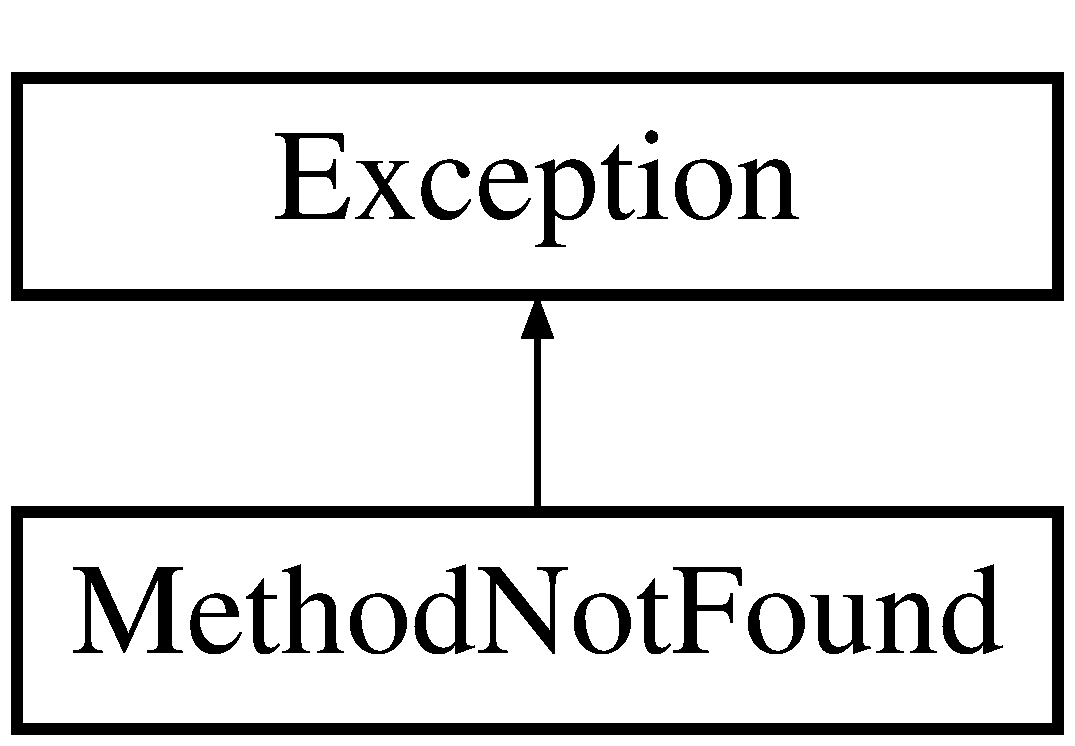
\includegraphics[height=2.000000cm]{class_method_not_found}
\end{center}
\end{figure}
\subsection*{Public Member Functions}
\begin{DoxyCompactItemize}
\item 
\hyperlink{class_method_not_found_a33a9e5d0643b4905247ec8270b4dd465}{\+\_\+\+\_\+construct} (\$title, \$message, \$code=0, Exception \$previous=null)
\item 
\hyperlink{class_method_not_found_a95e859a4588a39a1824b717378a84c29}{get\+Title} ()
\end{DoxyCompactItemize}
\subsection*{Protected Attributes}
\begin{DoxyCompactItemize}
\item 
\hyperlink{class_method_not_found_a5ef02115477cfad473df2455da5a908e}{\$title}
\end{DoxyCompactItemize}


\subsection{Detailed Description}


Definition at line 2 of file Method\+Not\+Found.\+php.



\subsection{Constructor \& Destructor Documentation}
\hypertarget{class_method_not_found_a33a9e5d0643b4905247ec8270b4dd465}{}\index{Method\+Not\+Found@{Method\+Not\+Found}!\+\_\+\+\_\+construct@{\+\_\+\+\_\+construct}}
\index{\+\_\+\+\_\+construct@{\+\_\+\+\_\+construct}!Method\+Not\+Found@{Method\+Not\+Found}}
\subsubsection[{\+\_\+\+\_\+construct}]{\setlength{\rightskip}{0pt plus 5cm}\+\_\+\+\_\+construct (
\begin{DoxyParamCaption}
\item[{}]{\$title, }
\item[{}]{\$message, }
\item[{}]{\$code = {\ttfamily 0}, }
\item[{Exception}]{\$previous = {\ttfamily null}}
\end{DoxyParamCaption}
)}\label{class_method_not_found_a33a9e5d0643b4905247ec8270b4dd465}
Initializes Exception


\begin{DoxyParams}[1]{Parameters}
string & {\em \$title} & \\
\hline
string & {\em \$message} & \\
\hline
int & {\em \$code} & \\
\hline
Exception & {\em \$previous} & \\
\hline
\end{DoxyParams}


Definition at line 16 of file Method\+Not\+Found.\+php.



References \$title.


\begin{DoxyCode}
16                                                                                          \{
17         $this->title = \hyperlink{class_method_not_found_a5ef02115477cfad473df2455da5a908e}{$title};
18         parent::\_\_construct($message, $code, $previous);
19     \}
\end{DoxyCode}


\subsection{Member Function Documentation}
\hypertarget{class_method_not_found_a95e859a4588a39a1824b717378a84c29}{}\index{Method\+Not\+Found@{Method\+Not\+Found}!get\+Title@{get\+Title}}
\index{get\+Title@{get\+Title}!Method\+Not\+Found@{Method\+Not\+Found}}
\subsubsection[{get\+Title}]{\setlength{\rightskip}{0pt plus 5cm}get\+Title (
\begin{DoxyParamCaption}
{}
\end{DoxyParamCaption}
)}\label{class_method_not_found_a95e859a4588a39a1824b717378a84c29}
Returns the title of the Exception

\begin{DoxyReturn}{Returns}
string \$title 
\end{DoxyReturn}


Definition at line 26 of file Method\+Not\+Found.\+php.



References \$title.


\begin{DoxyCode}
26                               \{
27         \textcolor{keywordflow}{return} \hyperlink{class_method_not_found_a5ef02115477cfad473df2455da5a908e}{$this->title};
28     \}
\end{DoxyCode}


\subsection{Field Documentation}
\hypertarget{class_method_not_found_a5ef02115477cfad473df2455da5a908e}{}\index{Method\+Not\+Found@{Method\+Not\+Found}!\$title@{\$title}}
\index{\$title@{\$title}!Method\+Not\+Found@{Method\+Not\+Found}}
\subsubsection[{\$title}]{\setlength{\rightskip}{0pt plus 5cm}string \$title\hspace{0.3cm}{\ttfamily [protected]}}\label{class_method_not_found_a5ef02115477cfad473df2455da5a908e}


Definition at line 6 of file Method\+Not\+Found.\+php.



Referenced by \+\_\+\+\_\+construct(), and get\+Title().



The documentation for this class was generated from the following file\+:\begin{DoxyCompactItemize}
\item 
C\+:/xampp/htdocs/mvc-\/framework/application/exceptions/\hyperlink{_method_not_found_8php}{Method\+Not\+Found.\+php}\end{DoxyCompactItemize}

\hypertarget{class_model_not_found}{}\section{Model\+Not\+Found Class Reference}
\label{class_model_not_found}\index{Model\+Not\+Found@{Model\+Not\+Found}}
Inheritance diagram for Model\+Not\+Found\+:\begin{figure}[H]
\begin{center}
\leavevmode
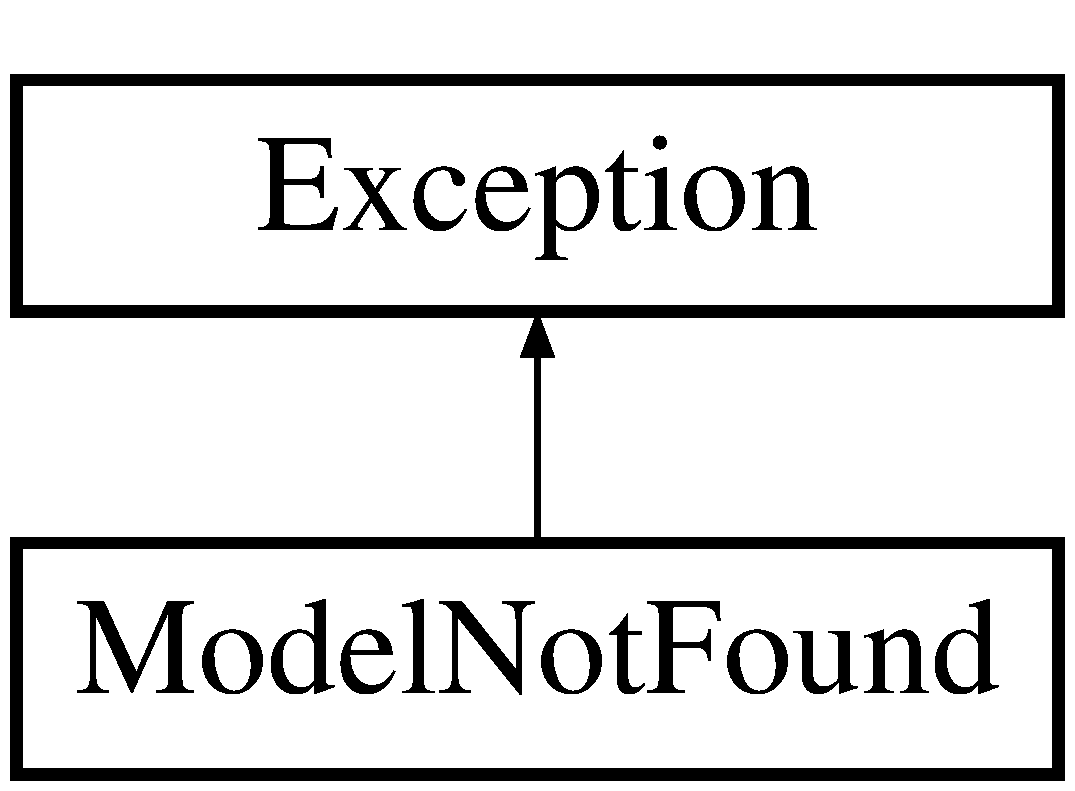
\includegraphics[height=2.000000cm]{class_model_not_found}
\end{center}
\end{figure}
\subsection*{Public Member Functions}
\begin{DoxyCompactItemize}
\item 
\hyperlink{class_model_not_found_a33a9e5d0643b4905247ec8270b4dd465}{\+\_\+\+\_\+construct} (\$title, \$message, \$code=0, Exception \$previous=null)
\item 
\hyperlink{class_model_not_found_a95e859a4588a39a1824b717378a84c29}{get\+Title} ()
\end{DoxyCompactItemize}
\subsection*{Protected Attributes}
\begin{DoxyCompactItemize}
\item 
\hyperlink{class_model_not_found_a5ef02115477cfad473df2455da5a908e}{\$title}
\end{DoxyCompactItemize}


\subsection{Detailed Description}


Definition at line 2 of file Model\+Not\+Found.\+php.



\subsection{Constructor \& Destructor Documentation}
\hypertarget{class_model_not_found_a33a9e5d0643b4905247ec8270b4dd465}{}\label{class_model_not_found_a33a9e5d0643b4905247ec8270b4dd465} 
\index{Model\+Not\+Found@{Model\+Not\+Found}!\+\_\+\+\_\+construct@{\+\_\+\+\_\+construct}}
\index{\+\_\+\+\_\+construct@{\+\_\+\+\_\+construct}!Model\+Not\+Found@{Model\+Not\+Found}}
\subsubsection{\texorpdfstring{\+\_\+\+\_\+construct()}{\_\_construct()}}
{\footnotesize\ttfamily \+\_\+\+\_\+construct (\begin{DoxyParamCaption}\item[{}]{\$title,  }\item[{}]{\$message,  }\item[{}]{\$code = {\ttfamily 0},  }\item[{Exception}]{\$previous = {\ttfamily null} }\end{DoxyParamCaption})}

Initializes Exception


\begin{DoxyParams}[1]{Parameters}
string & {\em \$title} & \\
\hline
string & {\em \$message} & \\
\hline
int & {\em \$code} & \\
\hline
Exception & {\em \$previous} & \\
\hline
\end{DoxyParams}


Definition at line 16 of file Model\+Not\+Found.\+php.



References \$title.


\begin{DoxyCode}
16                                                                                          \{
17         $this->title = \hyperlink{class_model_not_found_a5ef02115477cfad473df2455da5a908e}{$title};
18         parent::\_\_construct($message, $code, $previous);
19     \}
\end{DoxyCode}


\subsection{Member Function Documentation}
\hypertarget{class_model_not_found_a95e859a4588a39a1824b717378a84c29}{}\label{class_model_not_found_a95e859a4588a39a1824b717378a84c29} 
\index{Model\+Not\+Found@{Model\+Not\+Found}!get\+Title@{get\+Title}}
\index{get\+Title@{get\+Title}!Model\+Not\+Found@{Model\+Not\+Found}}
\subsubsection{\texorpdfstring{get\+Title()}{getTitle()}}
{\footnotesize\ttfamily get\+Title (\begin{DoxyParamCaption}{ }\end{DoxyParamCaption})}

Returns the title of the Exception

\begin{DoxyReturn}{Returns}
string \$title 
\end{DoxyReturn}


Definition at line 26 of file Model\+Not\+Found.\+php.



References \$title.


\begin{DoxyCode}
26                               \{
27         \textcolor{keywordflow}{return} \hyperlink{class_model_not_found_a5ef02115477cfad473df2455da5a908e}{$this->title};
28     \}
\end{DoxyCode}


\subsection{Field Documentation}
\hypertarget{class_model_not_found_a5ef02115477cfad473df2455da5a908e}{}\label{class_model_not_found_a5ef02115477cfad473df2455da5a908e} 
\index{Model\+Not\+Found@{Model\+Not\+Found}!\$title@{\$title}}
\index{\$title@{\$title}!Model\+Not\+Found@{Model\+Not\+Found}}
\subsubsection{\texorpdfstring{\$title}{$title}}
{\footnotesize\ttfamily string \$title\hspace{0.3cm}{\ttfamily [protected]}}



Definition at line 6 of file Model\+Not\+Found.\+php.



Referenced by \+\_\+\+\_\+construct(), and get\+Title().



The documentation for this class was generated from the following file\+:\begin{DoxyCompactItemize}
\item 
C\+:/xampp/htdocs/mvc-\/framework/application/exceptions/\hyperlink{_model_not_found_8php}{Model\+Not\+Found.\+php}\end{DoxyCompactItemize}

\hypertarget{class_user}{}\section{User Class Reference}
\label{class_user}\index{User@{User}}
\subsection*{Public Member Functions}
\begin{DoxyCompactItemize}
\item 
\hyperlink{class_user_a1797d3f80cc25452b4e97232ef14c6be}{get\+First\+Name} ()
\item 
\hyperlink{class_user_a3c626d0aca50df67aa89793615b7ffd1}{set\+First\+Name} (\$first\+Name)
\item 
\hyperlink{class_user_af0efc9a6afcaf0774ef627dbc4dbe43e}{get\+Last\+Name} ()
\item 
\hyperlink{class_user_acbe8bdd002179a3bc115ec7a9afb7e0b}{set\+Last\+Name} (\$last\+Name)
\item 
\hyperlink{class_user_a5a62afd4ce8cd694d7737b9ebbdd51d7}{get\+Age} ()
\item 
\hyperlink{class_user_a2c89f54beabff9157106c24878b70bca}{set\+Age} (\$age)
\item 
\hyperlink{class_user_acf082b95b344df14b9e8a6c09868dbcd}{get\+Email} ()
\item 
\hyperlink{class_user_a018ae17e436e09134922835cdd3235a7}{set\+Email} (\$email)
\item 
\hyperlink{class_user_acbf53279af16610c85d5f355860dd42b}{get\+Phone} ()
\item 
\hyperlink{class_user_a81a82307eef393fb41f0b3b76375472c}{set\+Phone} (\$phone)
\item 
\hyperlink{class_user_ab3d7e8f713f819b4121fb0bc38523c12}{\+\_\+\+\_\+to\+String} ()
\end{DoxyCompactItemize}


\subsection{Detailed Description}


Definition at line 2 of file User.\+php.



\subsection{Member Function Documentation}
\hypertarget{class_user_ab3d7e8f713f819b4121fb0bc38523c12}{}\label{class_user_ab3d7e8f713f819b4121fb0bc38523c12} 
\index{User@{User}!\+\_\+\+\_\+to\+String@{\+\_\+\+\_\+to\+String}}
\index{\+\_\+\+\_\+to\+String@{\+\_\+\+\_\+to\+String}!User@{User}}
\subsubsection{\texorpdfstring{\+\_\+\+\_\+to\+String()}{\_\_toString()}}
{\footnotesize\ttfamily User\+::\+\_\+\+\_\+to\+String (\begin{DoxyParamCaption}{ }\end{DoxyParamCaption})}



Definition at line 108 of file User.\+php.


\begin{DoxyCode}
108                                  \{
109         \textcolor{keywordflow}{return} $this->firstName . \textcolor{stringliteral}{' - '} . $this->lastName . \textcolor{stringliteral}{' - '} . $this->age . \textcolor{stringliteral}{' - '} . $this->email . \textcolor{stringliteral}{' -
       '} . $this->phone;
110     \}
\end{DoxyCode}
\hypertarget{class_user_a5a62afd4ce8cd694d7737b9ebbdd51d7}{}\label{class_user_a5a62afd4ce8cd694d7737b9ebbdd51d7} 
\index{User@{User}!get\+Age@{get\+Age}}
\index{get\+Age@{get\+Age}!User@{User}}
\subsubsection{\texorpdfstring{get\+Age()}{getAge()}}
{\footnotesize\ttfamily User\+::get\+Age (\begin{DoxyParamCaption}{ }\end{DoxyParamCaption})}



Definition at line 51 of file User.\+php.


\begin{DoxyCode}
51                             \{
52         \textcolor{keywordflow}{return} $this->age;
53     \}
\end{DoxyCode}
\hypertarget{class_user_acf082b95b344df14b9e8a6c09868dbcd}{}\label{class_user_acf082b95b344df14b9e8a6c09868dbcd} 
\index{User@{User}!get\+Email@{get\+Email}}
\index{get\+Email@{get\+Email}!User@{User}}
\subsubsection{\texorpdfstring{get\+Email()}{getEmail()}}
{\footnotesize\ttfamily User\+::get\+Email (\begin{DoxyParamCaption}{ }\end{DoxyParamCaption})}



Definition at line 72 of file User.\+php.


\begin{DoxyCode}
72                               \{
73         \textcolor{keywordflow}{return} $this->email;
74     \}
\end{DoxyCode}
\hypertarget{class_user_a1797d3f80cc25452b4e97232ef14c6be}{}\label{class_user_a1797d3f80cc25452b4e97232ef14c6be} 
\index{User@{User}!get\+First\+Name@{get\+First\+Name}}
\index{get\+First\+Name@{get\+First\+Name}!User@{User}}
\subsubsection{\texorpdfstring{get\+First\+Name()}{getFirstName()}}
{\footnotesize\ttfamily User\+::get\+First\+Name (\begin{DoxyParamCaption}{ }\end{DoxyParamCaption})}



Definition at line 9 of file User.\+php.


\begin{DoxyCode}
9                                   \{
10         \textcolor{keywordflow}{return} $this->firstName;
11     \}
\end{DoxyCode}
\hypertarget{class_user_af0efc9a6afcaf0774ef627dbc4dbe43e}{}\label{class_user_af0efc9a6afcaf0774ef627dbc4dbe43e} 
\index{User@{User}!get\+Last\+Name@{get\+Last\+Name}}
\index{get\+Last\+Name@{get\+Last\+Name}!User@{User}}
\subsubsection{\texorpdfstring{get\+Last\+Name()}{getLastName()}}
{\footnotesize\ttfamily User\+::get\+Last\+Name (\begin{DoxyParamCaption}{ }\end{DoxyParamCaption})}



Definition at line 30 of file User.\+php.


\begin{DoxyCode}
30                                  \{
31         \textcolor{keywordflow}{return} $this->lastName;
32     \}
\end{DoxyCode}
\hypertarget{class_user_acbf53279af16610c85d5f355860dd42b}{}\label{class_user_acbf53279af16610c85d5f355860dd42b} 
\index{User@{User}!get\+Phone@{get\+Phone}}
\index{get\+Phone@{get\+Phone}!User@{User}}
\subsubsection{\texorpdfstring{get\+Phone()}{getPhone()}}
{\footnotesize\ttfamily User\+::get\+Phone (\begin{DoxyParamCaption}{ }\end{DoxyParamCaption})}



Definition at line 90 of file User.\+php.


\begin{DoxyCode}
90                               \{
91         \textcolor{keywordflow}{return} $this->phone;
92     \}
\end{DoxyCode}
\hypertarget{class_user_a2c89f54beabff9157106c24878b70bca}{}\label{class_user_a2c89f54beabff9157106c24878b70bca} 
\index{User@{User}!set\+Age@{set\+Age}}
\index{set\+Age@{set\+Age}!User@{User}}
\subsubsection{\texorpdfstring{set\+Age()}{setAge()}}
{\footnotesize\ttfamily User\+::set\+Age (\begin{DoxyParamCaption}\item[{}]{\$age }\end{DoxyParamCaption})}



Definition at line 55 of file User.\+php.


\begin{DoxyCode}
55                                 \{
56         \textcolor{keywordflow}{if} (is\_null($age)) \{
57             \textcolor{keywordflow}{throw} \textcolor{keyword}{new} InvalidArgumentException(\textcolor{stringliteral}{'Age not allowed to be null!'});
58         \}
59         \textcolor{keywordflow}{if} (!is\_numeric($age)) \{
60             \textcolor{keywordflow}{throw} \textcolor{keyword}{new} InvalidArgumentException(\textcolor{stringliteral}{'Age not allowed to be string!'});
61         \}
62         \textcolor{keywordflow}{if} ($age < 13) \{
63             \textcolor{keywordflow}{throw} \textcolor{keyword}{new} OutOfRangeException(\textcolor{stringliteral}{'Age should be greater than 13!'});
64         \}
65         \textcolor{keywordflow}{if} ($age > 100) \{
66             \textcolor{keywordflow}{throw} \textcolor{keyword}{new} OutOfRangeException(\textcolor{stringliteral}{'Age should be lesser than 100!'});
67         \}
68 
69         $this->age = $age;
70     \}
\end{DoxyCode}
\hypertarget{class_user_a018ae17e436e09134922835cdd3235a7}{}\label{class_user_a018ae17e436e09134922835cdd3235a7} 
\index{User@{User}!set\+Email@{set\+Email}}
\index{set\+Email@{set\+Email}!User@{User}}
\subsubsection{\texorpdfstring{set\+Email()}{setEmail()}}
{\footnotesize\ttfamily User\+::set\+Email (\begin{DoxyParamCaption}\item[{}]{\$email }\end{DoxyParamCaption})}



Definition at line 76 of file User.\+php.


\begin{DoxyCode}
76                                     \{
77         \textcolor{keywordflow}{if} (is\_null($email)) \{
78             \textcolor{keywordflow}{throw} \textcolor{keyword}{new} InvalidArgumentException(\textcolor{stringliteral}{'Email not allowed to be null!'});
79         \}
80         \textcolor{keywordflow}{if} (filter\_var($email, FILTER\_VALIDATE\_EMAIL) === \textcolor{keyword}{false}) \{
81             \textcolor{keywordflow}{throw} \textcolor{keyword}{new} InvalidArgumentException(\textcolor{stringliteral}{'Email is not valid!'});
82         \}
83         \textcolor{keywordflow}{if} (strlen(utf8\_decode($email)) > 100) \{
84             \textcolor{keywordflow}{throw} \textcolor{keyword}{new} OutOfRangeException(\textcolor{stringliteral}{'Email should be lesser than 100 characters!'});
85         \}
86 
87         $this->email = $email;
88     \}
\end{DoxyCode}
\hypertarget{class_user_a3c626d0aca50df67aa89793615b7ffd1}{}\label{class_user_a3c626d0aca50df67aa89793615b7ffd1} 
\index{User@{User}!set\+First\+Name@{set\+First\+Name}}
\index{set\+First\+Name@{set\+First\+Name}!User@{User}}
\subsubsection{\texorpdfstring{set\+First\+Name()}{setFirstName()}}
{\footnotesize\ttfamily User\+::set\+First\+Name (\begin{DoxyParamCaption}\item[{}]{\$first\+Name }\end{DoxyParamCaption})}



Definition at line 13 of file User.\+php.


\begin{DoxyCode}
13                                             \{
14         \textcolor{keywordflow}{if} (is\_null($firstName)) \{
15             \textcolor{keywordflow}{throw} \textcolor{keyword}{new} InvalidArgumentException(\textcolor{stringliteral}{'First name not allowed to be null!'});
16         \}
17         \textcolor{keywordflow}{if} (is\_numeric($firstName)) \{
18             \textcolor{keywordflow}{throw} \textcolor{keyword}{new} InvalidArgumentException(\textcolor{stringliteral}{'First name not allowed to be int!'});
19         \}
20         \textcolor{keywordflow}{if} (strlen(utf8\_decode($firstName)) < 2) \{
21             \textcolor{keywordflow}{throw} \textcolor{keyword}{new} OutOfRangeException(\textcolor{stringliteral}{'First name should be greater than 2 characters!'});
22         \}
23         \textcolor{keywordflow}{if} (strlen(utf8\_decode($firstName)) > 100) \{
24             \textcolor{keywordflow}{throw} \textcolor{keyword}{new} OutOfRangeException(\textcolor{stringliteral}{'First name should be lesser than 100 characters!'});
25         \}
26 
27         $this->firstName = $firstName;
28     \}
\end{DoxyCode}
\hypertarget{class_user_acbe8bdd002179a3bc115ec7a9afb7e0b}{}\label{class_user_acbe8bdd002179a3bc115ec7a9afb7e0b} 
\index{User@{User}!set\+Last\+Name@{set\+Last\+Name}}
\index{set\+Last\+Name@{set\+Last\+Name}!User@{User}}
\subsubsection{\texorpdfstring{set\+Last\+Name()}{setLastName()}}
{\footnotesize\ttfamily User\+::set\+Last\+Name (\begin{DoxyParamCaption}\item[{}]{\$last\+Name }\end{DoxyParamCaption})}



Definition at line 34 of file User.\+php.


\begin{DoxyCode}
34                                           \{
35         \textcolor{keywordflow}{if} (is\_null($lastName)) \{
36             \textcolor{keywordflow}{throw} \textcolor{keyword}{new} InvalidArgumentException(\textcolor{stringliteral}{'Last name not allowed to be null!'});
37         \}
38         \textcolor{keywordflow}{if} (is\_numeric($lastName)) \{
39             \textcolor{keywordflow}{throw} \textcolor{keyword}{new} InvalidArgumentException(\textcolor{stringliteral}{'Last name not allowed to be int!'});
40         \}
41         \textcolor{keywordflow}{if} (strlen(utf8\_decode($lastName)) < 2) \{
42             \textcolor{keywordflow}{throw} \textcolor{keyword}{new} OutOfRangeException(\textcolor{stringliteral}{'Last name should be greater than 2 characters!'});
43         \}
44         \textcolor{keywordflow}{if} (strlen(utf8\_decode($lastName)) > 100) \{
45             \textcolor{keywordflow}{throw} \textcolor{keyword}{new} OutOfRangeException(\textcolor{stringliteral}{'Last name should be lesser than 100 characters!'});
46         \}
47 
48         $this->lastName = $lastName;
49     \}
\end{DoxyCode}
\hypertarget{class_user_a81a82307eef393fb41f0b3b76375472c}{}\label{class_user_a81a82307eef393fb41f0b3b76375472c} 
\index{User@{User}!set\+Phone@{set\+Phone}}
\index{set\+Phone@{set\+Phone}!User@{User}}
\subsubsection{\texorpdfstring{set\+Phone()}{setPhone()}}
{\footnotesize\ttfamily User\+::set\+Phone (\begin{DoxyParamCaption}\item[{}]{\$phone }\end{DoxyParamCaption})}



Definition at line 94 of file User.\+php.


\begin{DoxyCode}
94                                     \{
95         \textcolor{keywordflow}{if} (is\_null($phone)) \{
96             \textcolor{keywordflow}{throw} \textcolor{keyword}{new} InvalidArgumentException(\textcolor{stringliteral}{'Phone not allowed to be null!'});
97         \}   
98         \textcolor{keywordflow}{if} (strlen(utf8\_decode($phone)) < 8) \{
99             \textcolor{keywordflow}{throw} \textcolor{keyword}{new} OutOfRangeException(\textcolor{stringliteral}{'Phone should be greater than 7 characters!'});
100         \}
101         \textcolor{keywordflow}{if} (strlen(utf8\_decode($phone)) > 8) \{
102             \textcolor{keywordflow}{throw} \textcolor{keyword}{new} OutOfRangeException(\textcolor{stringliteral}{'Phone should be lesser than 9 characters!'});
103         \}
104 
105         $this->phone = $phone;
106     \}
\end{DoxyCode}


The documentation for this class was generated from the following file\+:\begin{DoxyCompactItemize}
\item 
C\+:/xampp/htdocs/mvc-\/framework/application/models/\hyperlink{_user_8php}{User.\+php}\end{DoxyCompactItemize}

\hypertarget{class_users}{}\section{Users Class Reference}
\label{class_users}\index{Users@{Users}}
Inheritance diagram for Users\+:\begin{figure}[H]
\begin{center}
\leavevmode
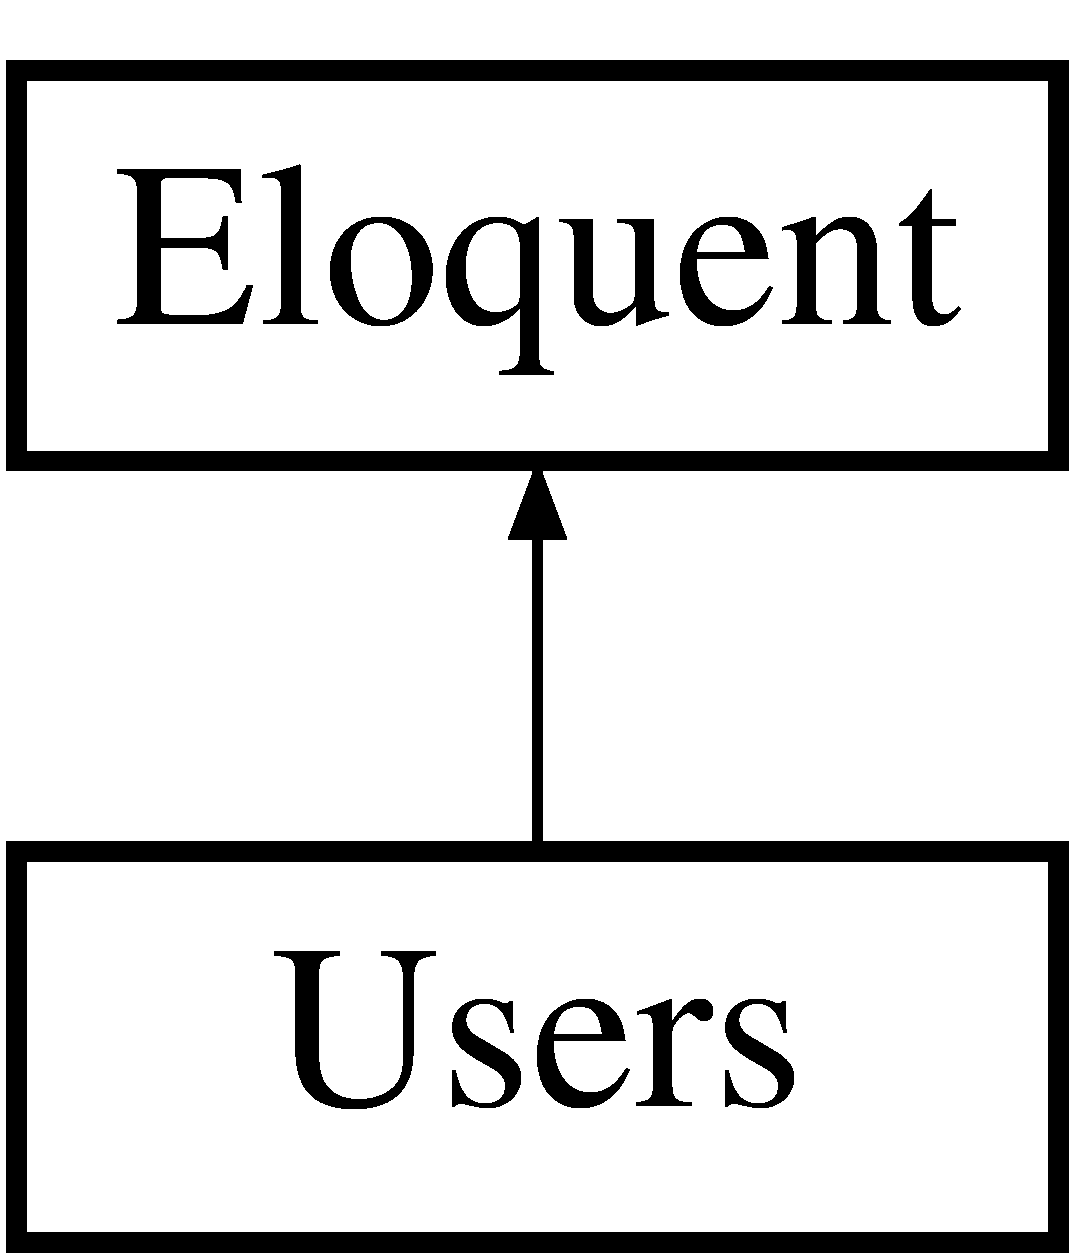
\includegraphics[height=2.000000cm]{class_users}
\end{center}
\end{figure}
\subsection*{Public Member Functions}
\begin{DoxyCompactItemize}
\item 
\hyperlink{class_users_a4a492898ef6d04f34f38e12fab5dcf57}{role} ()
\end{DoxyCompactItemize}
\subsection*{Protected Attributes}
\begin{DoxyCompactItemize}
\item 
\hyperlink{class_users_a6a90e74ccdf5efd70d51d10c906f8e32}{\$fillable} = \mbox{[}\textquotesingle{}user\+Name\textquotesingle{}, \textquotesingle{}password\textquotesingle{}, \textquotesingle{}first\+Name\textquotesingle{}, \textquotesingle{}last\+Name\textquotesingle{}, \textquotesingle{}age\textquotesingle{}, \textquotesingle{}avatar\textquotesingle{}, \textquotesingle{}email\textquotesingle{}, \textquotesingle{}phone\textquotesingle{}, \textquotesingle{}role\+Id\textquotesingle{}\mbox{]}
\end{DoxyCompactItemize}


\subsection{Detailed Description}


Definition at line 4 of file Users.\+php.



\subsection{Member Function Documentation}
\hypertarget{class_users_a4a492898ef6d04f34f38e12fab5dcf57}{}\index{Users@{Users}!role@{role}}
\index{role@{role}!Users@{Users}}
\subsubsection[{role}]{\setlength{\rightskip}{0pt plus 5cm}role (
\begin{DoxyParamCaption}
{}
\end{DoxyParamCaption}
)}\label{class_users_a4a492898ef6d04f34f38e12fab5dcf57}


Definition at line 7 of file Users.\+php.


\begin{DoxyCode}
8     \{
9         \textcolor{keywordflow}{return} $this->hasOne(\textcolor{stringliteral}{'Roles'}, \textcolor{stringliteral}{'id'});
10     \}
\end{DoxyCode}


\subsection{Field Documentation}
\hypertarget{class_users_a6a90e74ccdf5efd70d51d10c906f8e32}{}\index{Users@{Users}!\$fillable@{\$fillable}}
\index{\$fillable@{\$fillable}!Users@{Users}}
\subsubsection[{\$fillable}]{\setlength{\rightskip}{0pt plus 5cm}\$fillable = \mbox{[}\textquotesingle{}user\+Name\textquotesingle{}, \textquotesingle{}password\textquotesingle{}, \textquotesingle{}first\+Name\textquotesingle{}, \textquotesingle{}last\+Name\textquotesingle{}, \textquotesingle{}age\textquotesingle{}, \textquotesingle{}avatar\textquotesingle{}, \textquotesingle{}email\textquotesingle{}, \textquotesingle{}phone\textquotesingle{}, \textquotesingle{}role\+Id\textquotesingle{}\mbox{]}\hspace{0.3cm}{\ttfamily [protected]}}\label{class_users_a6a90e74ccdf5efd70d51d10c906f8e32}


Definition at line 5 of file Users.\+php.



The documentation for this class was generated from the following file\+:\begin{DoxyCompactItemize}
\item 
C\+:/xampp/htdocs/mvc-\/framework/application/models/\hyperlink{_users_8php}{Users.\+php}\end{DoxyCompactItemize}

\hypertarget{class_view_not_found}{}\section{View\+Not\+Found Class Reference}
\label{class_view_not_found}\index{View\+Not\+Found@{View\+Not\+Found}}
Inheritance diagram for View\+Not\+Found\+:\begin{figure}[H]
\begin{center}
\leavevmode
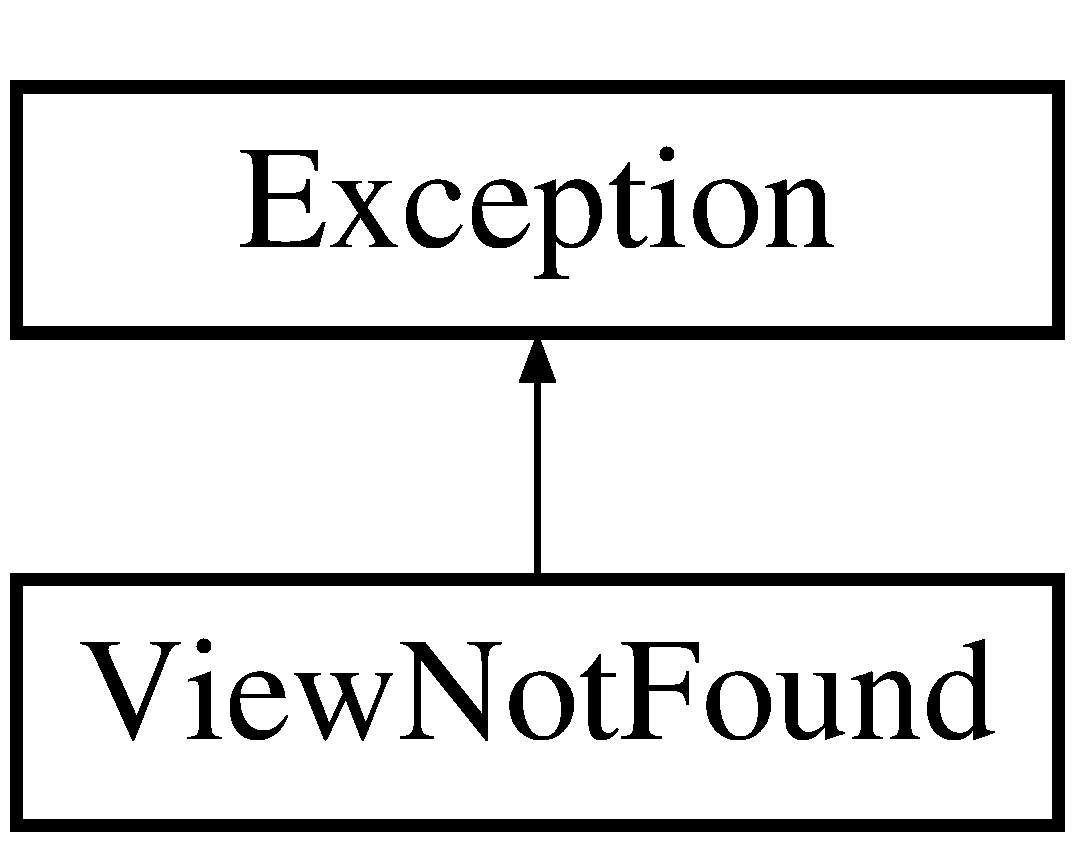
\includegraphics[height=2.000000cm]{class_view_not_found}
\end{center}
\end{figure}
\subsection*{Public Member Functions}
\begin{DoxyCompactItemize}
\item 
\hyperlink{class_view_not_found_a33a9e5d0643b4905247ec8270b4dd465}{\+\_\+\+\_\+construct} (\$title, \$message, \$code=0, Exception \$previous=null)
\item 
\hyperlink{class_view_not_found_a95e859a4588a39a1824b717378a84c29}{get\+Title} ()
\end{DoxyCompactItemize}
\subsection*{Protected Attributes}
\begin{DoxyCompactItemize}
\item 
\hyperlink{class_view_not_found_a5ef02115477cfad473df2455da5a908e}{\$title}
\end{DoxyCompactItemize}


\subsection{Detailed Description}


Definition at line 2 of file View\+Not\+Found.\+php.



\subsection{Constructor \& Destructor Documentation}
\hypertarget{class_view_not_found_a33a9e5d0643b4905247ec8270b4dd465}{}\index{View\+Not\+Found@{View\+Not\+Found}!\+\_\+\+\_\+construct@{\+\_\+\+\_\+construct}}
\index{\+\_\+\+\_\+construct@{\+\_\+\+\_\+construct}!View\+Not\+Found@{View\+Not\+Found}}
\subsubsection[{\+\_\+\+\_\+construct}]{\setlength{\rightskip}{0pt plus 5cm}\+\_\+\+\_\+construct (
\begin{DoxyParamCaption}
\item[{}]{\$title, }
\item[{}]{\$message, }
\item[{}]{\$code = {\ttfamily 0}, }
\item[{Exception}]{\$previous = {\ttfamily null}}
\end{DoxyParamCaption}
)}\label{class_view_not_found_a33a9e5d0643b4905247ec8270b4dd465}
Initializes Exception


\begin{DoxyParams}[1]{Parameters}
string & {\em \$title} & \\
\hline
string & {\em \$message} & \\
\hline
int & {\em \$code} & \\
\hline
Exception & {\em \$previous} & \\
\hline
\end{DoxyParams}


Definition at line 16 of file View\+Not\+Found.\+php.



References \$title.


\begin{DoxyCode}
16                                                                                          \{
17         $this->title = \hyperlink{class_view_not_found_a5ef02115477cfad473df2455da5a908e}{$title};
18         parent::\_\_construct($message, $code, $previous);
19     \}
\end{DoxyCode}


\subsection{Member Function Documentation}
\hypertarget{class_view_not_found_a95e859a4588a39a1824b717378a84c29}{}\index{View\+Not\+Found@{View\+Not\+Found}!get\+Title@{get\+Title}}
\index{get\+Title@{get\+Title}!View\+Not\+Found@{View\+Not\+Found}}
\subsubsection[{get\+Title}]{\setlength{\rightskip}{0pt plus 5cm}get\+Title (
\begin{DoxyParamCaption}
{}
\end{DoxyParamCaption}
)}\label{class_view_not_found_a95e859a4588a39a1824b717378a84c29}
Returns the title of the Exception

\begin{DoxyReturn}{Returns}
string \$title 
\end{DoxyReturn}


Definition at line 26 of file View\+Not\+Found.\+php.



References \$title.


\begin{DoxyCode}
26                               \{
27         \textcolor{keywordflow}{return} \hyperlink{class_view_not_found_a5ef02115477cfad473df2455da5a908e}{$this->title};
28     \}
\end{DoxyCode}


\subsection{Field Documentation}
\hypertarget{class_view_not_found_a5ef02115477cfad473df2455da5a908e}{}\index{View\+Not\+Found@{View\+Not\+Found}!\$title@{\$title}}
\index{\$title@{\$title}!View\+Not\+Found@{View\+Not\+Found}}
\subsubsection[{\$title}]{\setlength{\rightskip}{0pt plus 5cm}string \$title\hspace{0.3cm}{\ttfamily [protected]}}\label{class_view_not_found_a5ef02115477cfad473df2455da5a908e}


Definition at line 6 of file View\+Not\+Found.\+php.



Referenced by \+\_\+\+\_\+construct(), and get\+Title().



The documentation for this class was generated from the following file\+:\begin{DoxyCompactItemize}
\item 
C\+:/xampp/htdocs/mvc-\/framework/application/exceptions/\hyperlink{_view_not_found_8php}{View\+Not\+Found.\+php}\end{DoxyCompactItemize}

\chapter{File Documentation}
\hypertarget{boostrap_8php}{}\section{C\+:/xampp/htdocs/mvc-\/framework/application/boostrap.php File Reference}
\label{boostrap_8php}\index{C\+:/xampp/htdocs/mvc-\/framework/application/boostrap.\+php@{C\+:/xampp/htdocs/mvc-\/framework/application/boostrap.\+php}}
\subsection*{Variables}
\begin{DoxyCompactItemize}
\item 
foreach(glob(realpath(\+\_\+\+\_\+\+D\+I\+R\+\_\+\+\_\+). \textquotesingle{}/exceptions/$\ast$.php\textquotesingle{}) as \$exception) \hyperlink{boostrap_8php_a082ff60a5613c40db3435a164f1d4aca}{foreach} (glob(realpath(\+\_\+\+\_\+\+D\+I\+R\+\_\+\+\_\+). \textquotesingle{}/config/$\ast$.php\textquotesingle{}) as \$config)
\end{DoxyCompactItemize}


\subsection{Variable Documentation}
\hypertarget{boostrap_8php_a082ff60a5613c40db3435a164f1d4aca}{}\index{boostrap.\+php@{boostrap.\+php}!foreach@{foreach}}
\index{foreach@{foreach}!boostrap.\+php@{boostrap.\+php}}
\subsubsection[{foreach}]{\setlength{\rightskip}{0pt plus 5cm}foreach (glob(realpath(\+\_\+\+\_\+\+D\+I\+R\+\_\+\+\_\+). \textquotesingle{}/exceptions/$\ast$.php\textquotesingle{}) as \$exception) foreach(glob(realpath(\+\_\+\+\_\+\+D\+I\+R\+\_\+\+\_\+). \textquotesingle{}/config/$\ast$.php\textquotesingle{}) as \$config)}\label{boostrap_8php_a082ff60a5613c40db3435a164f1d4aca}
Bootstraps all the necessary files for the framework to work 

Definition at line 9 of file boostrap.\+php.


\hypertarget{config_8php}{}\section{C\+:/xampp/htdocs/mvc-\/framework/application/config/config.php File Reference}
\label{config_8php}\index{C\+:/xampp/htdocs/mvc-\/framework/application/config/config.\+php@{C\+:/xampp/htdocs/mvc-\/framework/application/config/config.\+php}}
\subsection*{Functions}
\begin{DoxyCompactItemize}
\item 
\hyperlink{config_8php_afeb1d281d402615776fdb0320a5b8d05}{initialize\+Config} ()
\end{DoxyCompactItemize}


\subsection{Function Documentation}
\hypertarget{config_8php_afeb1d281d402615776fdb0320a5b8d05}{}\label{config_8php_afeb1d281d402615776fdb0320a5b8d05} 
\index{config.\+php@{config.\+php}!initialize\+Config@{initialize\+Config}}
\index{initialize\+Config@{initialize\+Config}!config.\+php@{config.\+php}}
\subsubsection{\texorpdfstring{initialize\+Config()}{initializeConfig()}}
{\footnotesize\ttfamily initialize\+Config (\begin{DoxyParamCaption}{ }\end{DoxyParamCaption})}

Initialize config variables 

Definition at line 5 of file config.\+php.



Referenced by Application\textbackslash{}\+\_\+\+\_\+construct(), and Base\+Controller\textbackslash{}redirect\+Controller().


\begin{DoxyCode}
5                             \{
6     \textcolor{keywordflow}{return} [
7         \textcolor{stringliteral}{'defaultController'} => \textcolor{stringliteral}{'Basic'},
8         \textcolor{stringliteral}{'defaultMethod'} => \textcolor{stringliteral}{'index'},
9         \textcolor{stringliteral}{'defaultParameters'} => [],
10         \textcolor{stringliteral}{'defaultCharset'} => \textcolor{stringliteral}{'UTF-8'},
11         \textcolor{stringliteral}{'errorReporting'} => error\_reporting(E\_ALL)
12     ];
13 \}
\end{DoxyCode}

\hypertarget{database_8php}{}\section{C\+:/xampp/htdocs/mvc-\/framework/application/config/database.php File Reference}
\label{database_8php}\index{C\+:/xampp/htdocs/mvc-\/framework/application/config/database.\+php@{C\+:/xampp/htdocs/mvc-\/framework/application/config/database.\+php}}
\subsection*{Variables}
\begin{DoxyCompactItemize}
\item 
\hyperlink{database_8php_afe5d117e2943179b1ebb3fb365d3eb24}{\$capsule} = new Capsule()
\end{DoxyCompactItemize}


\subsection{Variable Documentation}
\hypertarget{database_8php_afe5d117e2943179b1ebb3fb365d3eb24}{}\index{database.\+php@{database.\+php}!\$capsule@{\$capsule}}
\index{\$capsule@{\$capsule}!database.\+php@{database.\+php}}
\subsubsection[{\$capsule}]{\setlength{\rightskip}{0pt plus 5cm}\$capsule = new Capsule()}\label{database_8php_afe5d117e2943179b1ebb3fb365d3eb24}
Initialize database variables 

Definition at line 7 of file database.\+php.


\hypertarget{controllers_2_basic_8php}{}\section{C\+:/xampp/htdocs/mvc-\/framework/application/controllers/\+Basic.php File Reference}
\label{controllers_2_basic_8php}\index{C\+:/xampp/htdocs/mvc-\/framework/application/controllers/\+Basic.\+php@{C\+:/xampp/htdocs/mvc-\/framework/application/controllers/\+Basic.\+php}}
\subsection*{Classes}
\begin{DoxyCompactItemize}
\item 
class \hyperlink{class_basic}{Basic}
\end{DoxyCompactItemize}

\hypertarget{views_2_basic_8php}{}\section{C\+:/xampp/htdocs/mvc-\/framework/application/views/basic.php File Reference}
\label{views_2_basic_8php}\index{C\+:/xampp/htdocs/mvc-\/framework/application/views/basic.\+php@{C\+:/xampp/htdocs/mvc-\/framework/application/views/basic.\+php}}

\hypertarget{_controller_not_found_8php}{}\section{C\+:/xampp/htdocs/mvc-\/framework/application/exceptions/\+Controller\+Not\+Found.php File Reference}
\label{_controller_not_found_8php}\index{C\+:/xampp/htdocs/mvc-\/framework/application/exceptions/\+Controller\+Not\+Found.\+php@{C\+:/xampp/htdocs/mvc-\/framework/application/exceptions/\+Controller\+Not\+Found.\+php}}
\subsection*{Classes}
\begin{DoxyCompactItemize}
\item 
class \hyperlink{class_controller_not_found}{Controller\+Not\+Found}
\end{DoxyCompactItemize}

\hypertarget{_method_not_found_8php}{}\section{C\+:/xampp/htdocs/mvc-\/framework/application/exceptions/\+Method\+Not\+Found.php File Reference}
\label{_method_not_found_8php}\index{C\+:/xampp/htdocs/mvc-\/framework/application/exceptions/\+Method\+Not\+Found.\+php@{C\+:/xampp/htdocs/mvc-\/framework/application/exceptions/\+Method\+Not\+Found.\+php}}
\subsection*{Data Structures}
\begin{DoxyCompactItemize}
\item 
class \hyperlink{class_method_not_found}{Method\+Not\+Found}
\end{DoxyCompactItemize}

\hypertarget{_model_not_found_8php}{}\section{C\+:/xampp/htdocs/mvc-\/framework/application/exceptions/\+Model\+Not\+Found.php File Reference}
\label{_model_not_found_8php}\index{C\+:/xampp/htdocs/mvc-\/framework/application/exceptions/\+Model\+Not\+Found.\+php@{C\+:/xampp/htdocs/mvc-\/framework/application/exceptions/\+Model\+Not\+Found.\+php}}
\subsection*{Classes}
\begin{DoxyCompactItemize}
\item 
class \hyperlink{class_model_not_found}{Model\+Not\+Found}
\end{DoxyCompactItemize}

\hypertarget{_view_not_found_8php}{}\section{C\+:/xampp/htdocs/mvc-\/framework/application/exceptions/\+View\+Not\+Found.php File Reference}
\label{_view_not_found_8php}\index{C\+:/xampp/htdocs/mvc-\/framework/application/exceptions/\+View\+Not\+Found.\+php@{C\+:/xampp/htdocs/mvc-\/framework/application/exceptions/\+View\+Not\+Found.\+php}}
\subsection*{Data Structures}
\begin{DoxyCompactItemize}
\item 
class \hyperlink{class_view_not_found}{View\+Not\+Found}
\end{DoxyCompactItemize}

\hypertarget{_application_8php}{}\section{C\+:/xampp/htdocs/mvc-\/framework/application/kernal/\+Application.php File Reference}
\label{_application_8php}\index{C\+:/xampp/htdocs/mvc-\/framework/application/kernal/\+Application.\+php@{C\+:/xampp/htdocs/mvc-\/framework/application/kernal/\+Application.\+php}}
\subsection*{Classes}
\begin{DoxyCompactItemize}
\item 
class \hyperlink{class_application}{Application}
\end{DoxyCompactItemize}

\hypertarget{_base_controller_8php}{}\section{C\+:/xampp/htdocs/mvc-\/framework/application/kernal/\+Base\+Controller.php File Reference}
\label{_base_controller_8php}\index{C\+:/xampp/htdocs/mvc-\/framework/application/kernal/\+Base\+Controller.\+php@{C\+:/xampp/htdocs/mvc-\/framework/application/kernal/\+Base\+Controller.\+php}}
\subsection*{Classes}
\begin{DoxyCompactItemize}
\item 
class \hyperlink{class_base_controller}{Base\+Controller}
\end{DoxyCompactItemize}

\hypertarget{_user_8php}{}\section{C\+:/xampp/htdocs/mvc-\/framework/application/models/\+User.php File Reference}
\label{_user_8php}\index{C\+:/xampp/htdocs/mvc-\/framework/application/models/\+User.\+php@{C\+:/xampp/htdocs/mvc-\/framework/application/models/\+User.\+php}}
\subsection*{Data Structures}
\begin{DoxyCompactItemize}
\item 
class \hyperlink{class_user}{User}
\end{DoxyCompactItemize}

\hypertarget{_users_8php}{}\section{C\+:/xampp/htdocs/mvc-\/framework/application/models/\+Users.php File Reference}
\label{_users_8php}\index{C\+:/xampp/htdocs/mvc-\/framework/application/models/\+Users.\+php@{C\+:/xampp/htdocs/mvc-\/framework/application/models/\+Users.\+php}}
\subsection*{Data Structures}
\begin{DoxyCompactItemize}
\item 
class \hyperlink{class_users}{Users}
\end{DoxyCompactItemize}

\hypertarget{basic__base_8php}{}\section{C\+:/xampp/htdocs/mvc-\/framework/application/views/layout/basic\+\_\+base.php File Reference}
\label{basic__base_8php}\index{C\+:/xampp/htdocs/mvc-\/framework/application/views/layout/basic\+\_\+base.\+php@{C\+:/xampp/htdocs/mvc-\/framework/application/views/layout/basic\+\_\+base.\+php}}

\hypertarget{basic__detail_8php}{}\section{C\+:/xampp/htdocs/mvc-\/framework/application/views/layout/basic\+\_\+detail.php File Reference}
\label{basic__detail_8php}\index{C\+:/xampp/htdocs/mvc-\/framework/application/views/layout/basic\+\_\+detail.\+php@{C\+:/xampp/htdocs/mvc-\/framework/application/views/layout/basic\+\_\+detail.\+php}}

%--- End generated contents ---

% Index
\backmatter
\newpage
\phantomsection
\clearemptydoublepage
\addcontentsline{toc}{chapter}{Index}
\printindex

\end{document}
